\documentclass[../main.tex]{subfiles}
\begin{document}
\chapter{Python Data Structures}

\section{Introduction}
Python is object-oriented programming language where each object is implemented using \texttt{C++} in the backend. The built-in data types of \texttt{C++} follows more rigidly to the abstract data structures. We would get by just learning how to use Python data types alone: its \textbf{property}--immutable or mutable, its \textbf{built-in in-place operations}--such as \texttt{append()}, \texttt{insert()}, \texttt{add()}, \texttt{remove()}, \texttt{replace()} and so, and \textbf{built-in functions} and \textbf{operations} that offers additional ability to manipulate data structure--an object here. However, some data types' behaviors might confuse us with abstract data structures, making it hard to access and evaluate its efficiency. 

In this chapter and the following three chapters, we starts to learn Python data structures by relating its \texttt{C++} data structures to our learned abstract data structures, and then introduce each's property, built-in operations, built-in functions and operations. \textit{Please read the section Understanding Object in the Appendix--Python Knowledge Base to to study the properties of Built-in Data Types first if Python is not your familiar language}.

\paragraph{Python Built-in Data Types} In Python 3, we have four built-in scalar data types: \texttt{int}, \texttt{float}, \texttt{complex}, \texttt{bool}. At higher level, it includes four sequence types: \texttt{str}--string type, \texttt{list}, \texttt{tuple}, and \texttt{range}; one mapping type: \texttt{dict} and two set types: \texttt{set} and \texttt{fronzenset}. Among these 12 built-in data types, other than the scalar types, the others representing some of our introduced abstract data structures. 


\paragraph{Abstract Data Types with Python Data Types/Modules}
To relate the abstract data types to our build-in data types we have:
\begin{itemize}
    \item Sequence type corresponds to Array data structure: includes \texttt{string}, \texttt{list}, \texttt{tuple}, and \texttt{range}
    \item \texttt{dict}, \texttt{set}, and \texttt{fronzenset} mapps to the hash tables.
    \item For linked list, stack, queue, we either need to implement it with build-in data types or we have Python Modules. 
\end{itemize}
%%%%%%%%%%%%%%%%
% Array : list, string, and tuple! %
%%%%%%%%%%%%%%%%
% \chapter{Basic Data Structure}
\section{Array and Python Sequence}
\label{chapter_array_string}
 We will see from other remaining contents of this part that how array-based Python data structures are used to implement the other data structures. On the LeetCode, these two data structures are involved into $25\%$ of LeetCode Problems. 
\subsection{Introduction to Python Sequence}
In Python, \textit{sequences} are defined as ordered sets of objects indexed by non-negative integers, we use \textit{index} to refer and in Python it defaultly starts at $0$. Sequence types are \textbf{iterable}. Iterables are able to be iterated over. Iterators are the agents that perform the iteration, where we have \texttt{iter()} built-in function. 
\begin{itemize}
    \item \texttt{string} is  a sequence of characters, it is immutable, and with \textbf{static array} as its backing data structure in C++. 
    \item \texttt{list} and \texttt{tuple} are sequences of \textbf{arbitrary} objects.--meaning it accepts different types of objects including the 12 built-in data types and any other objects. This sounds fancy and like magic! However, it does not change the fact that its backing abstract data structure is \textbf{dynamic array}. They are able to have arbitrary type of objects through the usage of pointers to objects, pointing to object's physical location, and each pointer takes fixed number of bytes in space (in 32-bit system, 4 bytes, and for a 64-bit system, 8 bytes instead). 
    \item \texttt{range}: In Python 3, \texttt{range()} is a type. But range does not have backing array data structure to save a sequence of value, it computes on demand. Thus we will first introduce range and get done with it before we focus on other sequence types. 
\begin{lstlisting}[language=Python]
>>> type(range)
<class 'type'>
\end{lstlisting}
    \end{itemize}

All these sequence type data structures share the most common methods and operations shown in Table~\ref{tab:common_method_sequence_python} and \ref{tab:common_operation_sequence_python}. To note that in Python, the indexing starts from 0. 

Let us examine each type of sequence further to understand its performance, and relation to array data structures. 
%%%%%%%%%%%%%%%%%%%%%%%%%%%%%%%%%%%%STring%%%%%%%%%%%%%%%
\subsection{Range}
\subsubsection{Range Syntax}
The range object has three attributes: \texttt{start}, \texttt{stop}, \texttt{step}, and a range object can be created as \texttt{range(start, stop, step}. These attributes need to integers--both negative and positive works--to define a range, which will be $[start, stop)$. The default value for \texttt{start} and \texttt{stop} is 0.  For example:
\begin{lstlisting}[language=Python]
>>> a = range(10)
>>> b = range(0, 10, 2)
>>> a, b
(range(0, 10), range(0, 10, 2))
\end{lstlisting}
Now, we print it out:
\begin{lstlisting}[language=Python]
>>> for i in a:
...     print(i, end=' ')
... 
0 1 2 3 4 5 6 7 8 9
\end{lstlisting}
And for \texttt{b}, it will be:
\begin{lstlisting}[language=Python]
>>> for i in b:
...     print(i, end=' ')
... 
0 2 4 6 8
\end{lstlisting}
Like any other sequence types, \texttt{range} is iterable, can be indexed and sliced. 
\begin{lstlisting}[language=Python]
\end{lstlisting}
\subsubsection{What you do not see}
The range object might be a little bizarre when we first learn it. Is it an iterator, a generator? The answer to both questions are NO. What is it then? It is more like a sequence type that differs itself without other counterparts with its own unique properties: 
\begin{itemize}
    \item It is ``lazy'' in the sense that it doesn’t generate every number that it ``contain'' when we create it. Instead it gives those numbers to us as we need them when looping over it. Thus, it saves us space:
\begin{lstlisting}[language=Python]
>>> a = range(1_000_000)
>>> b = [i for i in a]
>>> a.__sizeof__(), b.__sizeof__()
(48, 8697440)
\end{lstlisting}
This is just how we define the behavior of the range class back in the C++ code. We does not need to save all integers in the range, but be generated with function that specifically asks for it. 
    \item It is not an iterator; it won't get consumed. We can iterate it multiple times. This is understandable given how it is implemented.
\end{itemize}
%%%%%%%%%%%%%%%%%%%%%%%%%%%%%%%%%%%%STring%%%%%%%%%%%%%%%
\subsection{String}
String is \textbf{static array} and its items are just characters, represented using  ASCII or Unicode \footnote{In Python 3, all strings are represented in Unicode. In Python 2 are stored internally as 8-bit ASCII, hence it is required to attach 'u' to make it Unicode. It is no longer necessary now.}. String is immutable which means once its created we can no longer modify its content or extent its size. String is more compact compared with storing the characters in \texttt{list} because of its backing array wont be assigned to any extra space.

\subsubsection{String Syntax} strings can be created in Python by wrapping a sequence of characters in single or double quotes. Multi-line strings can easily be created using three quote characters.

\paragraph{New a String}


We specially introduce some commonly and useful functions. 
\paragraph{Join}
The \texttt{str.join()} method will concatenate two strings, but in a way that passes one string through another.  For example, we can  use the \texttt{str.join()} method to add whitespace to that string, which we can do like so:
\begin{lstlisting}[language=Python]
balloon = "Sammy has a balloon."
print(" ".join(balloon))
#Ouput
S a m m y   h a s   a   b a l l o o n .
\end{lstlisting}
The \texttt{str.join()} method is also useful to combine a list of strings into a new single string.
\begin{lstlisting}[language=Python]
print(",".join(["a", "b", "c"]))
#Ouput
abc
\end{lstlisting}
\paragraph{Split}
Just as we can join strings together, we can also split strings up using the \texttt{str.split()} method. This method separates the string by whitespace if no other parameter is given.
\begin{lstlisting}[language=Python]
print(balloon.split())
#Ouput
['Sammy', 'has', 'a', 'balloon.']
\end{lstlisting}
We can also use str.split() to remove certain parts of an original string. For example, let’s remove the letter 'a' from the string:
\begin{lstlisting}[language=Python]
print(balloon.split("a"))
#Ouput
['S', 'mmy h', 's ', ' b', 'lloon.']
\end{lstlisting}
Now the letter a has been removed and the strings have been separated where each instance of the letter a had been, with whitespace retained.

\paragraph{Replace}The \texttt{str.replace()} method can take an original string and return an updated string with some replacement.

Let’s say that the balloon that Sammy had is lost. Since Sammy no longer has this balloon, we will change the substring "has" from the original string balloon to "had" in a new string:
\begin{lstlisting}[language=Python]
print(balloon.replace("has","had"))
#Ouput
Sammy had a balloon.
\end{lstlisting}
We can use the replace method to delete a substring:
\begin{lstlisting}[language=Python]
ballon.replace("has", '')
\end{lstlisting}
Using the string methods \texttt{str.join()}, \texttt{str.split()}, and \texttt{str.replace()} will provide you with greater control to manipulate strings in Python.

\paragraph{Conversion between Integer and Character}
Function \texttt{ord()} would get the int value (ASCII) of the char. And in case you want to convert back after playing with the number, function \texttt{chr()} does the trick.
\begin{lstlisting}[language = Python]
print(ord('A'))# Given a string of length one, return an integer representing the Unicode  code point of the character when the argument is a unicode object,
print(chr(65))
\end{lstlisting}

\subsubsection{String Functions}
 Because string is one of the most fundamental built-in data types, this makes managing its built-in common methods shown in Table~\ref{tab:common_operation_string} and \ref{tab:common_operation_string_boolean} necessary.  Use boolean methods to check whether characters are lower case, upper case, or title case, can help us to sort our data appropriately, as well as provide us with the opportunity to standardize data we collect by checking and then modifying strings as needed. 
\begin{table}[!ht]
\begin{small}
\centering
\noindent\captionof{table}{ Common Methods of String}
 \noindent \begin{tabular}{|p{0.45\columnwidth}|p{0.55\columnwidth}| }
  \hline
Method & Description   \\ \hline
count(substr, [start, end])  & Counts the occurrences of a substring with optional start and end position \\\hline
find(substr, [start, end])  &Returns the index of the first occurrence of a substring or returns -1 if the substring is not found\\ \hline
join(t)  &Joins the strings in sequence t with current string between each item\\ \hline
lower()/upper() &Converts the string to all lowercase or uppercase\\ \hline
replace(old, new) &Replaces old substring with new substring\\ \hline
strip([characters]) &Removes withspace or optional characters\\ \hline
split([characters], [maxsplit]) &Splits a string separated by whitespace or an optional separator. Returns a list\\ \hline
expandtabs([tabsize]) & Replaces tabs with spaces.
\end{tabular}
  \label{tab:common_operation_string}
  
  \centering
\noindent\captionof{table}{ Common Boolean Methods of String}
 \noindent \begin{tabular}{|p{0.45\columnwidth}|p{0.55\columnwidth}| }
  \hline
Boolean Method & Description   \\ \hline

isalnum() &	String consists of only alphanumeric characters (no symbols)\\ \hline
isalpha() &	String consists of only alphabetic characters (no symbols)\\ \hline
islower() &	String's alphabetic characters are all lower case\\ \hline
isnumeric() & String consists of only numeric characters\\ \hline
isspace() &	String consists of only whitespace characters\\ \hline
istitle() &	String is in title case\\ \hline
isupper() &	String's alphabetic characters are all upper case\\ \hline
\end{tabular}
  \label{tab:common_operation_string_boolean}
  \end{small}
\end{table}



%%%%%%%%%%%%%%%%%%%List%%%%%%%%%%%%%%%%%%%%%%%%%%%%%%%%%%
\subsection{List}
The underlying abstract data structure of \texttt{list} data types is \textbf{dynamic array}, meaning we can add, delete, modify items in the list. It supports random access by indexing.  List is the most widely one among sequence types due to its mutability. 

 Even if list supports data of arbitrary types, we do not prefer to do this. Use \texttt{tuple} or \texttt{namedtuple} for better practice and offers better clarification. 
\subsubsection{What You see: List Syntax}
\textbf{New a List:} We have multiple ways to new either empty list or with initialized data. List comprehension is an elegant and concise way to create new list from an existing list in Python.
\begin{lstlisting}[language = Python]
# new an empty list
lst = []
lst2 = [2, 2, 2, 2] # new a list with initialization
lst3 = [3]*5     # new a list size 5 with 3 as initialization
print(lst, lst2, lst3)
# output
# [] [2, 2, 2, 2] [3, 3, 3, 3, 3] 
\end{lstlisting}

We can use \textbf{list comprehension} and use \texttt{enumerate} function to loop over its items.
\begin{lstlisting}[language=Python]
lst1 = [3]*5     # new a list size 5 with 3 as initialization
lst2 = [4 for i in range(5)]
for idx, v in enumerate(lst1):
    lst1[idx] += 1
\end{lstlisting}

\paragraph{Search} We use method \texttt{list.index()} to obtain the index of the searched item. 
\begin{lstlisting}[language = Python]
print(lst.index(4)) #find 4, and return the index
# output
# 3 
\end{lstlisting}
If we print(lst.index(5)) will raise ValueError: 5 is not in list. Use the following code instead.
\begin{lstlisting}[language=Python]
if 5 in lst:
    print(lst.index(5))
\end{lstlisting}
\textbf{Add Item } We can add items into list through \texttt{insert(index, value)}--inserting an item at a position in the original list or \texttt{list.append(value)}--appending an item at the end of the list. 
\begin{lstlisting}[language = Python]
# INSERTION
lst.insert(0, 1) # insert an element at index 0, and since it is empty lst.insert(1, 1) has the same effect
print(lst)

lst2.insert(2, 3)
print(lst2)
# output
# [1]
# [2, 2, 3, 2, 2]
# APPEND
for i in range(2, 5):
    lst.append(i)
print(lst)
# output
# [1, 2, 3, 4]
\end{lstlisting}

\textbf{Delete Item} 

\textbf{Get Size of the List} We can use \texttt{len} built-in function to find out the number of items storing in the list. 
\begin{lstlisting}[language=Python]
print(len(lst2))
# 4
\end{lstlisting}




%%%%%%%%%%%%%%%%%%%%%%%%%%%%%List and Array%%%%%%%%%%%%%%%%%%%%%%%%%%%%%%
\subsubsection{What you do not see: Understand List}
To understand list, we need start with its C++ implementation, we do not introduce the C++ source code, but instead use function to access and evaluate its property. 
\paragraph{List Object and Pointers} In a 64-bits (8 bytes) system, such as in Google Colab, a pointer is represented with 8 bytes space. In Python3, the list object itself takes $64$ bytes in space. And any additional element takes $8$ bytes. In Python, we can use \texttt{getsizeof()} from \texttt{sys} module to get its memory size, for example:
\begin{lstlisting}[language=Python]
lst_lst = [[], [1], ['1'], [1, 2], ['1', '2']]
\end{lstlisting}
And now, let us get the memory size of \texttt{lst\_lst} and each list item in this list.
\begin{lstlisting}[language=Python]
import sys
for lst in lst_lst:
  print(sys.getsizeof(lst), end=' ')
print(sys.getsizeof(lst_lst))
\end{lstlisting}
The output is:
\begin{lstlisting}[numbers=none]
64 72 72 80 80 104
\end{lstlisting}
We can see a list of integers takes the same memory size as of a list of strings with equal length.
\paragraph{insert and append} Whenever insert and append is called, and assume the original length is $n$, Python could compare $n+1$ with its allocated length. If you append or insert to a Python list and the backing array isn't big enough, the backing array must be expanded. When this happens, the backing array is grown by approximately 12\% the following formula (comes from C++):
\begin{lstlisting}[language=C]
new_allocated = (size_t)newsize + (newsize >> 3) +
    (newsize < 9 ? 3 : 6);
\end{lstlisting}
Do an experiment, we can see how it works. Here we use \texttt{id()} function to obtain the pointer's physical address. We compare the size of the list and its underlying backing array's real additional size in space (with 8 bytes as unit).
\begin{lstlisting}[language=Python]
a = []
for size in range(17):
  a.insert(0, size)
  print('size:', len(a), 'bytes:', (sys.getsizeof(a)-64)//8, 'id:', id(a))
\end{lstlisting}
The output is:
\begin{lstlisting}[numbers=none]
size: 1 bytes: 4 id: 140682152394952
size: 2 bytes: 4 id: 140682152394952
size: 3 bytes: 4 id: 140682152394952
size: 4 bytes: 4 id: 140682152394952
size: 5 bytes: 8 id: 140682152394952
size: 6 bytes: 8 id: 140682152394952
size: 7 bytes: 8 id: 140682152394952
size: 8 bytes: 8 id: 140682152394952
size: 9 bytes: 16 id: 140682152394952
size: 10 bytes: 16 id: 140682152394952
size: 11 bytes: 16 id: 140682152394952
size: 12 bytes: 16 id: 140682152394952
size: 13 bytes: 16 id: 140682152394952
size: 14 bytes: 16 id: 140682152394952
size: 15 bytes: 16 id: 140682152394952
size: 16 bytes: 16 id: 140682152394952
size: 17 bytes: 25 id: 140682152394952
\end{lstlisting}
The output addresses the growth patterns as [0, 4, 8, 16, 25, 35, 46, 58, 72, 88, ...]. 

Amortizely, \texttt{append} takes $O(1)$. However, it is $O(n)$ for \texttt{insert} because it has to first shift all items in the original list from [pos, end] by one position, and put the item at pos with random access. 

\subsubsection{Common Methods of List} We have already seen how to use \texttt{append}, \texttt{insert}. Now, Table~\ref{tab:common_operation_list} shows us the common List Methods, and they will be used as \texttt{list.methodName()}.
\begin{table}[h]
\begin{small}
\centering
\noindent\captionof{table}{ Common Methods of List}
 \noindent \begin{tabular}{|p{0.45\columnwidth}|p{0.55\columnwidth}| }
  \hline
Method & Description   \\ \hline
append()  & Add an element to the end of the list \\\hline
extend(l)  &Add all elements of a list to the another list\\ \hline
insert(index, val)  &Insert an item at the defined index $s$\\ \hline
pop(index)  &Removes and returns an element at the given index\\ \hline
remove(val) & Removes an item from the list\\ \hline
clear()  &Removes all items from the list\\ \hline
index(val) &Returns the index of the first matched item\\ \hline
count(val) &Returns the count of number of items passed as an argument\\ \hline
sort() &Sort items in a list in ascending order\\ \hline
reverse() &Reverse the order of items in the list (same as list[::-1])\\ \hline
copy() &Returns a shallow copy of the list (same as list[::])\\ \hline
\end{tabular}
  \label{tab:common_operation_list}
  \end{small}
\end{table}


\subsubsection{Two-dimensional List}
Two dimensional list is a list within a list.  In this type of array the position of an data element is referred by two indices instead of one. So it represents a table with rows and columns of data. For example, we can declare the following 2-d array:
\begin{lstlisting}[language=Python]
ta = [[11, 3, 9, 1], [25, 6,10], [10, 8, 12, 5]]
\end{lstlisting}
The scalar data in two dimensional lists can be accessed using two indices. One index referring to the main or parent array and another index referring to the position of the data  in the inner list. If we mention only one index then the entire inner list is printed for that index position. The example below illustrates how it works. 
\begin{lstlisting}[language=Python]
print(ta[0])
print(ta[2][1])
\end{lstlisting}
And with the output
\begin{lstlisting}[numbers=none]
[11, 3, 9, 1]
8
\end{lstlisting}
In the above example, we new a 2-d list and initialize them with values. There are also ways to new an empty 2-d array or fix the dimension of the outer array and leave it empty for the inner arrays:
\begin{lstlisting}[language=Python]
# empty two dimensional list
empty_2d = [[]]

# fix the outer dimension
fix_out_d = [[] for _ in range(5)]
print(fix_out_d)
\end{lstlisting}
All the other operations such as delete, insert, update are the same as of the one-dimensional list. 

\paragraph{Matrices} We are going to need the concept of matrix, which is defined as a collection of numbers arranged into a fixed number of rows and columns. For example, we define $3 \times  4$ (read as 3 by 4) order matrix is a set of numbers arranged in 3 rows and 4 columns. And for $m_1$ and $m_2$, they are doing the same things. 
\begin{lstlisting}[language=Python]
rows, cols = 3, 4
m1 = [[0 for _ in range(cols)] for _ in range(rows)] # rows * cols
m2 = [[0]*cols for _ in range(rows)] # rows * cols
print(m1, m2)
\end{lstlisting}
The output is:
\begin{lstlisting}[numbers=none]
[[0, 0, 0, 0], [0, 0, 0, 0], [0, 0, 0, 0]] [[0, 0, 0, 0], [0, 0, 0, 0], [0, 0, 0, 0]] 
\end{lstlisting}
We assign value to m1 and m2 at index (1, 2) with value $1$:
\begin{lstlisting}[language=Python]
m1[1][2] = 1
m2[1][2] = 1
print(m1, m2)
\end{lstlisting}
And the output is:
\begin{lstlisting}[numbers=none]
[[0, 0, 0, 0], [0, 0, 1, 0], [0, 0, 0, 0]] [[0, 0, 0, 0], [0, 0, 1, 0], [0, 0, 0, 0]]
\end{lstlisting}
However, we can not declare it in the following way, because we end up with some copies of the same inner lists, thus modifying one element in the inner lists will end up changing all of the them in the corresponding positions. Unless the feature suits the situation.
\begin{lstlisting}[language=Python]
# wrong declaration
m4 = [[0]*cols]*rows
m4[1][2] = 1
print(m4)
\end{lstlisting}
With output:
\begin{lstlisting}[numbers=none]
[[0, 0, 1, 0], [0, 0, 1, 0], [0, 0, 1, 0]
\end{lstlisting}

\paragraph{Access Rows and Columns} In the real problem solving, we might need to access rows and columns.  Accessing rows is quite easy since it follows the declaraion of two-dimensional array.  
\begin{lstlisting}[language=Python]
# accessing row
for row in m1:
  print(row)
\end{lstlisting}
With the output:
\begin{lstlisting}[numbers=none]
[0, 0, 0, 0]
[0, 0, 1, 0]
[0, 0, 0, 0]
\end{lstlisting}
However, accessing columns will be less straightforward. To get each column, we need another inner for loop or list comprehension through all rows and obtain the value from that column. This is usually a lot slower than accessing each row due to the fact that each row is a pointer while each col we need to obtain from each row. 
\begin{lstlisting}[language=Python]
# accessing col
for i in range(cols):
    col = [row[i] for row in m1]
    print(col)
\end{lstlisting}
The output is:
\begin{lstlisting}[numbers=none]
[0, 0, 0]
[0, 0, 0]
[0, 1, 0]
[0, 0, 0]
\end{lstlisting}
There's also a handy ``idiom'' for transposing a nested list, turning 'columns' into 'rows':
\begin{lstlisting}[language=Python]
transposedM1 = list(zip(*m1))
print(transposedM1)
\end{lstlisting}
The output will be:
\begin{lstlisting}[numbers=none]
[(0, 0, 0), (0, 0, 0), (0, 1, 0), (0, 0, 0)]
\end{lstlisting}

% \begin{bclogo}[couleur = blue!30, arrondi=0.1,logo=\bccrayon,ombre=true]{Try use \texttt{numpy} third party module?} 
% \begin{lstlisting}[language=Python]
% import numpy as np
% b = np.array(list) # convert list to array
% col = b[:, 0] # access the first col
% row = b[0, :] # access the first row
% \end{lstlisting}
% \end{bclogo}

\subsection{Tuple}
A \texttt{tuple} has \textbf{static array} as its backing abstract data structure in C, which is immutable--we can not add, delete, or replace items once its created and assigned with value. You might think if \texttt{list} is a dynamic array and has no restriction same as of the tuple, why would we need \texttt{tuple} then? 

\paragraph{Tuple VS List} We list how we use each data type and why is it.  The main benefit of tuple's immutability is it is hashable, we can use them as keys in the hash table--\texttt{dictionary types}, whereas the mutable types such as list and range can not be applied. Besides, in the case that the data does not to change, the tuple's immutability will guarantee that the data remains write-protected and iterating an immutable sequence is faster than a mutable sequence, giving it slight performance boost. Also, we generally use tuple to store a variety of data types. For example, in a class score system, for a student, we might want to have its name, student id, and test score, we can write \texttt{('Bob', 12345, 89)}. 



\subsubsection{Tuple Syntax}
\paragraph{New and Initialize Tuple} Tuples are created by separating the items with a comma. It is commonly wrapped in parentheses for better readability. Tuple can also be created via a built-in function \texttt{tuple()}, if the argument to \texttt{tuple()} is a sequence then this creates a tuple of elements of that sequences. This is also used to realize type conversion. 

An empty tuple: 
\begin{lstlisting}[language=Python]
tup = ()
tup3 = tuple() 
\end{lstlisting}
When there is only one item, put comma behind so that it wont be translated as \texttt{string}, which is a bit bizarre!
\begin{lstlisting}[language=Python]
tup2 = ('crack', )
tup1 = ('crack', 'leetcode', 2018, 2019)
\end{lstlisting}
Converting a string to a tuple with each character separated.
\begin{lstlisting}[language=Python]
tup4 = tuple("leetcode") # the sequence is passed as a tuple of elements
>> tup4:  ('l', 'e', 'e', 't', 'c', 'o', 'd', 'e') 
\end{lstlisting}
Converting a list to a tuple.
\begin{lstlisting}[language=Python]
tup5 = tuple(['crack', 'leetcode', 2018, 2019]) # same as tuple1
\end{lstlisting}
If we print out these tuples, it will be
\begin{lstlisting}
tup1:  ('crack', 'leetcode', 2018, 2019) 
tup2:  crack 
tup3:  () 
tup4:  ('l', 'e', 'e', 't', 'c', 'o', 'd', 'e') 
tup5:  ('crack', 'leetcode', 2018, 2019)
\end{lstlisting}

\paragraph{Changing a Tuple} Assume we have the following tuple:
\begin{lstlisting}[language=Python]
tup = ('a', 'b', [1, 2, 3])
\end{lstlisting}
If we want to change it to \texttt{('c', 'b', [4,2,3])}. We can not do the following operation as we said a tuple cannot be changed in-place once it has been assigned. 
\begin{lstlisting}[language=Python]
tup = ('a', 'b', [1, 2, 3])
#tup[0] = 'c' #TypeError: 'tuple' object does not support item assignment
\end{lstlisting}
Instead, we initialize another tuple and assign it to \texttt{tup} variable.
\begin{lstlisting}[language=Python]
tup=('c', 'b', [4,2,3])
\end{lstlisting}
However, for its items which are mutable itself, we can still manipulate it. For example,  we can use index to access the list item at the last position of a tuple and modify the list.
\begin{lstlisting}[language=Python]
tup[-1][0] = 4
#('a', 'b', [4, 2, 3])
\end{lstlisting}


% \paragraph{Deleting a Tuple} Because tuple is immutable, it also means we cannot delete or remove items from a tuple. But deleting a tuple entirely is possible using the keyword \texttt{del}. 
% \begin{lstlisting}[language=Python]
% del tup
% print(tup)
% \end{lstlisting}
% After del, when try to use tup again it returns NameError. 
% \begin{lstlisting}
% NameError: name 'tup' is not defined
% \end{lstlisting}
\subsubsection{Understand Tuple}
The backing structure is \textbf{static array} which states that the way the tuple is structure is similar to list, other than its write-protected. We will just brief on its property.
\paragraph{Tuple Object and Pointers} Tuple object itself takes $48$ bytes. And all the others are similar to corresponding section in list.
\begin{lstlisting}[language=Python]
lst_tup = [(), (1,), ('1',), (1, 2), ('1', '2')]
import sys
for tup in lst_tup:
  print(sys.getsizeof(tup), end=' ')
\end{lstlisting}
The output will be:
\begin{lstlisting}[numbers=none]
48 56 56 64 64 
\end{lstlisting}

\subsubsection{Named Tuples}In named tuple, we can give all records a name, say ``Computer\_Science'' to indicate the class name, and we give each item a name, say 'name', 'id', and 'score'. We need to import \texttt{namedtuple} class  from module \texttt{collections}. For example:
\begin{lstlisting}[language=Python]
record1 = ('Bob', 12345, 89)
from collections import namedtuple
Record = namedtuple('Computer_Science', 'name id score')
record2 = Record('Bob', id=12345, score=89)
print(record1, record2)
\end{lstlisting}
The output will be:
\begin{lstlisting}[language=Python]
('Bob', 12345, 89) Computer_Science(name='Bob', id=12345, score=89)
\end{lstlisting}






\subsection{Summary}
All these sequence type data structures share the most common methods and operations shown in Table~\ref{tab:common_method_sequence_python} and \ref{tab:common_operation_sequence_python}. To note that in Python, the indexing starts from 0. 
\begin{table}[h]
\begin{small}
\centering
\noindent\captionof{table}{ Common Methods for Sequence Data Type in Python}
 \noindent \begin{tabular}{|p{0.45\columnwidth}|p{0.55\columnwidth}| }
  \hline
 Function Method& Description   \\ \hline
len(s)  & Get the size of sequence s \\\hline
min(s, [,default=obj, key=func])  &The minimum value in s (alphabetically for strings)\\ \hline
max(s, [,default=obj, key=func])  &The maximum value in s (alphabetically for strings)\\ \hline
 sum(s, [,start=0)  &The sum of elements in s(return $TypeError$ if $s$ is not numeric)\\ \hline
all(s)  & Return $True$ if all elements in $s$ are True (Similar to $and$)\\ \hline
any(s)  &Return $True$ if any element in $s$ is True (similar to $or$)\\ \hline
\end{tabular}
  \label{tab:common_method_sequence_python}
\centering
\noindent\captionof{table}{ Common out of place operators for Sequence Data Type in Python}
 \noindent \begin{tabular}{|p{0.45\columnwidth}|p{0.55\columnwidth}| }
  \hline
Operation & Description   \\ \hline
s + r  & Concatenates two sequences of the same type \\\hline
s * n  &Make $n$ copies of $s$, where $n$ is an integer\\ \hline
$v_1, v_2, ..., v_n = s$  &Unpack $n$ variables from $s$\\ \hline
s[i]  &Indexing-returns $i$th element of $s$\\ \hline
s[i:j:stride]  & Slicing-returns elements between $i$ and $j$ with optinal stride\\ \hline
x in s  &Return $True$ if element $x$ is in $s$\\ \hline
x not in s  &Return $True$ if element $x$ is not in $s$\\ \hline
\end{tabular}
  \label{tab:common_operation_sequence_python}
  \end{small}
\end{table}



%%%%%%%%%%%%%%%%
% Circular Array! %
%%%%%%%%%%%%%%%%
\subsection{Bonus} 
\paragraph{Circular Array}
The corresponding problems include:
\begin{enumerate}
    \item 503. Next Greater Element II
\end{enumerate}


\subsection{Exercises }
\begin{enumerate}
    \item 985. Sum of Even Numbers After Queries (easy)
    \item 937. Reorder Log Files

You have an array of logs.  Each log is a space delimited string of words.

For each log, the first word in each log is an alphanumeric identifier.  Then, either:

    Each word after the identifier will consist only of lowercase letters, or;
    Each word after the identifier will consist only of digits.

We will call these two varieties of logs letter-logs and digit-logs.  It is guaranteed that each log has at least one word after its identifier.

Reorder the logs so that all of the letter-logs come before any digit-log.  The letter-logs are ordered lexicographically ignoring identifier, with the identifier used in case of ties.  The digit-logs should be put in their original order.

Return the final order of the logs.
\begin{lstlisting}
Example 1:

Input: ["a1 9 2 3 1","g1 act car","zo4 4 7","ab1 off key dog","a8 act zoo"]
Output: ["g1 act car","a8 act zoo","ab1 off key dog","a1 9 2 3 1","zo4 4 7"]

 

Note:

    0 <= logs.length <= 100
    3 <= logs[i].length <= 100
    logs[i] is guaranteed to have an identifier, and a word after the identifier.
\end{lstlisting}
\begin{lstlisting}[language=Python]
def reorderLogFiles(self, logs):
    letters = []
    digits = []
    for idx, log in enumerate(logs):
        splited = log.split(' ')
        id = splited[0]
        type = splited[1]
        
        if type.isnumeric():
            digits.append(log)
        else:
            letters.append((' '.join(splited[1:]), id))
    letters.sort() #default sorting by the first element and then the second in the tuple
        
    return [id + ' ' + other for other, id in letters] + digits
\end{lstlisting}
\begin{lstlisting}[language=Python]
def reorderLogFiles(logs):
    digit = []
    letters = []
    info = {}
    for log in logs:
        if '0' <= log[-1] <= '9':
            digit.append(log)
        else:
            letters.append(log)
            index = log.index(' ')
            info[log] = log[index+1:]

    letters.sort(key= lambda x: info[x])
    return letters + digit
\end{lstlisting}
\end{enumerate}

%%%%%%%%%%%%%%%%%%%%%%%%%%%%%%%%%%%%%%%%%%%%%%%%%%%%%%%%%%%%%%%%%%%%%%%%%%%%%%%%
% Linked List
%%%%%%%%%%%%%%%%%%%%%%%%%%%%%%%%%%%%%%%%%%%%%%%%%%%%%%%%%%%%%%%%%%%%%%%%%%%%%%%%%%%
\section{Linked List}
\label{chapter_linked_list}
Python does not have built-in data type or modules that offers the Linked List-like data structures, however, it is not hard to implement it ourselves.  
%%%%%%%%%%Singly Linked List%%%%%%%%%%%%
\subsection{Singly Linked List}
\label{linked_list_subsec_singly}
\begin{figure}[h!]
    \centering
    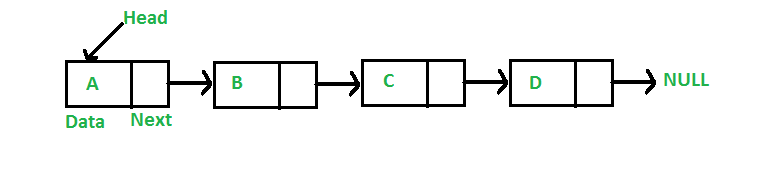
\includegraphics[width=.98\columnwidth]{fig/linked_list1.png}
    \caption{Linked List Structure}
    \label{fig:singly_linkedlist}
\end{figure}

Linked list consists of \texttt{nodes}, and each \texttt{node} consists of at least two  variables for singly linked lit: \texttt{val} to save data and \texttt{next}, a pointer  that points to the successive node. The \texttt{Node} class is given as:
\begin{lstlisting}[language=Python]
class Node(object):
     def __init__(self, val = None):
         self.val = val
         self.next = None
\end{lstlisting}

In Singly Linked List, usually we can start to with a \textbf{head} node which points to the first node in the list; only with this single node we are able to trace other nodes. For simplicity, demonstrate the process without using class, but we provide a class implementation with name \texttt{SinglyLinkeList} in our online python source code. Now, let us create an empty node named \texttt{head}.
\begin{lstlisting}[language=Python]
head = None
\end{lstlisting}
We need to implement its standard operations, including insertion/append, delete, search, clear. However, if we allow to the head node to be \texttt{None}, there would be special cases to handle. Thus, we implement a \textbf{dummy node}--a node but with \texttt{None} as its value as the head, to simplify the coding. Thus, we point the head to a dummy node: 
\begin{lstlisting}[language=Python]
head = Node(None)
\end{lstlisting}
\paragraph{Append Operation} As the append function in list, we add node at the very end of the linked list. If without the dummy node, then there will be two cases: 
\begin{itemize}
    \item When \texttt{head} is an empty node, we  assign the new \texttt{node} to \texttt{head}.
    \item When it is not empty, we because all we have that is available is the head pointer, thus, it we need to first traverse all the nodes up till the very last node whose \texttt{next} is \texttt{None}, then we connect \texttt{node} to the last node through assigning it to the last node's \texttt{next} pointer.
\end{itemize}
The first case is simply bad: we would generate a new node and we can not track the head through in-place operation. However, with the dummy node, only the second case will appear. The code is: 
\begin{lstlisting}[language=Python]
def append(head, val):
  node = Node(val)
  cur = head
  while cur.next:
    cur = cur.next
  cur.next = node
  return
\end{lstlisting}
Now, let use create the same exact linked list in Fig.~\ref{fig:singly_linkedlist}:
\begin{lstlisting}[language=Python]
for val in ['A', 'B', 'C', 'D']:
  append(head, val)
\end{lstlisting}
\paragraph{Generator and Search Operations} In order to traverse and iterate the linked list using syntax like \texttt{for ... in} statement like any other sequence data types in Python, we implement the \texttt{gen()} function that returns a generator of all nodes of the list. Because we have a dummy node, so we always start at \texttt{head.next}.
\begin{lstlisting}[language=Python]
def gen(head):
    cur = head.next
    while cur:
      yield cur
      cur = cur.next
\end{lstlisting}
Now, let us print out the linked list we created:
\begin{lstlisting}[language=Python]
for node in iter(head):
  print(node.val, end = ' ')
\end{lstlisting}
Here is the output:
\begin{lstlisting}[numbers=none]
A B C D 
\end{lstlisting}
Search operation we find a node by value, and we return this node, otherwise, we return \texttt{None}.
\begin{lstlisting}[language=Python]
def search(head, val):
  for node in gen(head):
    if node.val == val:
      return node
  return None
\end{lstlisting}
Now, we search for value `B' with:
\begin{lstlisting}[language=Python]
node = search(head, 'B')
\end{lstlisting}

\paragraph{Delete Operation} For deletion, there are two scenarios: deleting a node by value when we are given the head node and deleting a given node such as the node we got from searching 'B'.

The first case requires us to first locate the node first, and rewire the pointers between the predecessor and successor of the deleting node. Again here, if we do not have a dummy node, we would have two cases: if the node is the head node, repoint the head to the next node,   we connect the previous node to deleting node's next node, and the head pointer remains untouched. With dummy node, we would only have the second situation. In the process, we use an additional variable \texttt{prev} to track the predecessor. 
\begin{lstlisting}[language=Python]
def delete(head, val):
    cur = head.next # start from dummy node
    prev = head
    while cur:
        if cur.val == val:
            # rewire
            prev.next = cur.next
            return
        prev = cur
        cur = cur.next
\end{lstlisting}
Now, let us delete one more node--'A' with this function.
\begin{lstlisting}[language=Python]
delete(head,'A')
for n in gen(head):
  print(n.val, end = ' ')
\end{lstlisting}
Now the output will indicate we only have two nodes left:
\begin{lstlisting}[language=Python]
C D 
\end{lstlisting}

The  second case might seems a bit impossible--we do not know its previous node, the trick we do is to copy the value of the next node to current node, and we delete the next node instead by pointing current node to the node after next node. While, that is only when the deleting node is not the last node. When it is, we have no way to completely delete it; but we can make it ``invalid'' by setting value and  \texttt{Next} to \texttt{None}.
\begin{lstlisting}[language=Python]
def delete(head, val):
    cur = head.next # start from dummy node
    prev = head
    while cur:
        if cur.val == val:
            # rewire
            prev.next = cur.next
            return
        prev = cur
        cur = cur.next
\end{lstlisting}
Now, let us try deleting the node 'B' via our previously found \texttt{node}.
\begin{lstlisting}[language=Python]
deleteByNode(node)
for n in gen(head):
  print(n.val, end = ' ')
\end{lstlisting}
The output is:
\begin{lstlisting}[language=Python]
A C D 
\end{lstlisting}

\paragraph{Clear} When we need to clear all the nodes of the linked list, we just set the node next to the dummy head to \texttt{None}.
\begin{lstlisting}[language=Python]
    def clear(self):
        self.head = None
        self.size = 0
\end{lstlisting}

Question: Some linked list can only allow insert node at the tail which is Append, some others might allow insertion at any location. To get the length of the linked list easily in O(1), we need a variable to track the size


\subsection{Doubly Linked List}
\label{linked_list_subsec_doubly}
\begin{figure}[h]
    \centering
    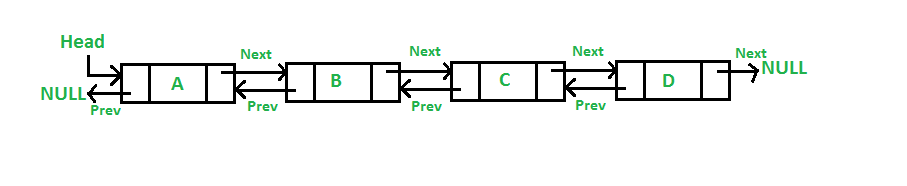
\includegraphics[width=0.9\columnwidth]{fig/DLL1.png}
    \caption{Doubly Linked List}
    \label{fig:dll1}
\end{figure}
On the basis of Singly linked list, doubly linked list (dll) contains an extra pointer in the node structure which is typically called \texttt{prev} (short for previous) and points back to its predecessor in the list. We define the \texttt{Node} class as:
\begin{lstlisting}[language=Python]
class Node: 
    def __init__(self, val, prev = None, next = None): 
        self.val = val 
        self.prev = prev # reference to previous node in DLL
        self.next = next # reference to next node in DLL 
\end{lstlisting}
Similarly, let us start with setting the dummy node as head:
\begin{lstlisting}[language=Python]
head = Node()
\end{lstlisting}

Now, instead of for me to continue to implement all operations that are slightly variants of the singly linked list, why do not you guys implement it? Do not worry, try it first, and also I have the answer covered in the google colab, enjoy!

Now, I assume that you have implemented those operations and or checked up the solutions. We would notice in \texttt{search()} and \texttt{gen()}, the code is exactly the same, and for other operations, there is only one or two lines of code that differs from SLL. Let's quickly list these operations: 

\paragraph{Append Operation} In DLL, we have to set the appending node's \texttt{prev} pointer to the last node of the linked list. The code is: 
\begin{lstlisting}[language=Python]
def append(head, val):
  node = Node(val)
  cur = head
  while cur.next:
    cur = cur.next
  cur.next = node
  node.prev = cur ## only difference
  return
\end{lstlisting}

\paragraph{Generator and Search Operations} There is no much difference if we just search through \texttt{next} pointer. However, with the extra \texttt{prev} pointer, we can have two options: either search forward through \texttt{next} or backward through \texttt{prev} if the given starting node is any node. Whereas for SLL, this is not an option, because we would not be able to conduct a complete search--we can only search among the items behind from the given node. When the data is ordered in some way, or if the program is parallel--situations that bidirectional search would make sense.
\begin{lstlisting}[language=Python]
def gen(head):
    cur = head.next
    while cur:
      yield cur
      cur = cur.next
\end{lstlisting}
\begin{lstlisting}[language=Python]
def search(head, val):
  for node in gen(head):
    if node.val == val:
      return node
  return None
\end{lstlisting}

\paragraph{Delete Operation} 
To delete a node by value, we first find it in the linked list, and the rewiring process needs to deal with the next node's \texttt{prev} pointer if the next node exists.
\begin{lstlisting}[language=Python]
def delete(head, val):
    cur = head.next # start from dummy node
    while cur:
        if cur.val == val:
            # rewire
            cur.prev.next = cur.next
            if cur.next:
              cur.next.prev = cur.prev
            return
        cur = cur.next
\end{lstlisting}
For \texttt{deleteByNode}, because we are cutting off \texttt{node.next}, we need to connect node to \texttt{node.next.next} in two directions: first point \texttt{prev} of later node to current node, and set point current node's \texttt{next} to the later node.
\begin{lstlisting}[language=Python]
def deleteByNode(node):
  # pull the next node to current node
  if node.next:
    node.val = node.next.val
    if node.next.next:
      node.next.next.prev = node
    node.next = node.next.next
  else: #last node
    node.prev.next = None
    return node
\end{lstlisting}

\paragraph{Comparison} We can see there is some slight advantage of dll over sll, but it comes with the cost of handing the extra \texttt{prev}. This would only be an advantage when bidirectional searching plays dominant factor in the matter of efficiency, otherwise, better stick with sll. 

\paragraph{Tips} From our implementation, in some cases we still need to worry about if it is the last node or not. The coding logic can further be simplified if we put a dummy node at the end of the linked list too.



\subsection{Bonus}
% \paragraph{Tail Pointer}
% For both singly and doubly linked list, if we add another \textbf{tail} pointer to its class, which points at the last node in the list, can simplify some operations of the linked list from $O(n)$ to $O(1)$. 

\paragraph{Circular Linked List}
A circular linked list is a variation of linked list in which the first node connects to last node. To make a circular linked list from a normal linked list: in singly linked list, we simply set the last node's \texttt{next} pointer to the first node; in doubly linked list, other than setting the last node's \texttt{next} pointer, we set the \texttt{prev} pointer of the first node to the last node making the circular in both directions. 

Compared with a normal linked list, circular linked list saves time for us to go to the first node from the last (both sll and dll) or go to the last node from the first node (in dll) by doing it in a single step through the extra connection. Because it is a circle, when ever a search with a \texttt{while} loop is needed, we  need to make sure the end condition: just make sure we searched a whole cycle by comparing the iterating node to the starting node. 

\paragraph{Recursion} Recursion offers additional pass of traversal--bottom-up on the basis of the top-down direction and in practice, it offers clean and simpler code compared with iteration. 

\subsection{Hands-on Examples}
\paragraph{Remove Duplicates (L83)} Given a sorted linked list, delete all duplicates such that each element appear only once.
\begin{lstlisting}[numbers=none]
Example 1:

Input: 1->1->2
Output: 1->2

Example 2:

Input: 1->1->2->3->3
Output: 1->2->3
\end{lstlisting}

\subsubsection{Analysis} This is a linear complexity problem, the most straightforward way is to iterate through the linked list and compare the current node's value with the next's to check its equivalency: (1) if YES: delete one of the nodes, here we go for the next node; (2) if NO: we can move to the next node safely and sound.

\paragraph{Iteration without Dummy Node} We start from the \texttt{head} in a \texttt{while} loop, if the next node exists and if the value equals, we delete next node. However, after the deletion, we can not move to next directly; say if we have 1->1->1, when the second 1 is removed, if we move, we will be at the last 1, and would fail removing all possible duplicates. The code is given:
\begin{lstlisting}[language=Python]
def deleteDuplicates(self, head):
    """
    :type head: ListNode
    :rtype: ListNode
    """
    if not head:
        return None
    
   def iterative(head):
        current = head
        while current:
            if current.next and current.val == current.next.val:
                # delete next
                current.next = current.next.next
            else:   
                current = current.next
        return head
    
    return iterative(head)
\end{lstlisting}
\paragraph{With Dummy Node} We see with a dummy node, we put \texttt{current.next} in the whole loop, because only if the next node exists, would we need to compare the values. Besides, we do not need to check this condition within the \texttt{while} loop. 
\begin{lstlisting}[language=Python]
def iterative(head):
    dummy = ListNode(None)
    dummy.next = head
    current = dummy
    while current.next:
        if current.val == current.next.val:
            # delete next
            current.next = current.next.next
        else:   
            current = current.next
    return head
\end{lstlisting}
\paragraph{ Recursion}Now, if we use recursion and return the node, thus, at each step, we can compare our node with the returned node (locating behind the current node), same logical applies. A better way to help us is drawing out an example. With 1->1->1. The last 1 will return, and at the second last 1, we can compare them, because it equals, we delete the last 1, now we backtrack to the first 1 with the second last 1 as returned node, we compare again. The code is the simplest among all solutions. 
\begin{lstlisting}[language=Python]
 def recursive(node):
        if node.next is None:
            return node
        
        next = recursive(node.next)
        if next.val == node.val:
            node.next = node.next.next
        return node
\end{lstlisting}



\subsection{Exercises}
Basic operations:
\begin{enumerate}
    \item 237. Delete Node in a Linked List (easy, delete only given current node)
    \item 2. Add Two Numbers (medium)
    \item 92. Reverse Linked List II (medium, reverse in one pass)
    \item 83. Remove Duplicates from Sorted List (easy)
    \item 82. Remove Duplicates from Sorted List II (medium)
    \item Sort List
    \item Reorder List
\end{enumerate}

Fast-slow pointers:
\begin{enumerate}
    \item 876. Middle of the Linked List (easy)
    \item Two Pointers in Linked List
    \item Merge K Sorted Lists
\end{enumerate}

Recursive and linked list:
\begin{enumerate}
\item 369. Plus One Linked List (medium)
\end{enumerate}





% this is the advanced data structure

%%%%%%%%%%%%%%%%%%%%%%%%%%%%%%%%%%%%%%%%%%%%%%%%%%%%%%%%%%%%%%%%%%%%%%%%%%%%%%%%%%%%%
%%%%%%%%%%%%% stack and queue
%%%%%%%%%%%%%%%%%%%%%%%%%%%%%%%%%%%%%%%%%%%%%%%%%%%%%%%%%%%%%%%%%%%%%%%%%%%%%%%%%%%%%%%%%
\section{Stack and Queue}
\label{chapter_queue_stack}
Stack data structures fits well for tasks that require us to check the previous states from cloest level to furtherest level. Here are some examplary applications: (1) reverse an array, (2) implement DFS iteratively as we will see in Chapter~\ref{chapter_non_linear_searching}, (3) keep track of the return address during function calls, (4) recording the previous states for backtracking algorithms. 

Queue data structures can be used: (1) implement BFS shown in Chapter~\ref{chapter_non_linear_searching}, (2) implement queue buffer. 

In the remaining section, we will discuss the implement with the built-in data types or using built-in modules.  After this, we will learn more advanced queue and stack: the priority queue and the monotone queue which can be used to solve medium to hard problems on LeetCode.

\subsection{Basic Implementation}

For Queue and Stack data structures, the essential operations are  two that adds and removes item. In Stack, they are usually called \textbf{PUSH} and \textbf{POP}. PUSH will add one item, and POP will remove one item and return its value. These two operations should only take $O(1)$ time. Sometimes, we need another operation called PEEK which just return the element that can be accessed in the queue or stack without removing it. While in Queue, they are named as \textbf{Enqueue} and \textbf{Dequeue}.

The simplest implementation is to use Python List by function $insert()$ (insert an item at appointed position), $pop()$ (removes the element at the given index, updates the list , and return the value. The default is to remove the last item), and $append()$.  However, the list data structure can not meet the time complexity requirement as these operations can potentially take $O(n)$. We feel its necessary because the code is simple thus saves you from using the specific module or implementing a more complex one.  

\paragraph{Stack} The implementation for stack is simplily adding and deleting element from the end. 
\begin{lstlisting}[language = Python]
# stack
s = []
s.append(3)
s.append(4)
s.append(5)
s.pop()
\end{lstlisting}

\paragraph{Queue} For queue, we can append at the last, and pop from the first index always. Or we can insert at the first index, and use pop the last element.
\begin{lstlisting}[language = Python]
# queue 
# 1: use append and pop
q = []
q.append(3)
q.append(4)
q.append(5)
q.pop(0)
\end{lstlisting}
Running the above code will give us the following output:
\begin{lstlisting}[language=Python]
print('stack:', s, ' queue:', q)
stack: [3, 4]  queue: [4, 5]
\end{lstlisting}

The other way to implement it is to write class and implement them using concept of node which shares the same definition as the linked list node. Such implementation can satisfy the $O(1)$ time restriction. For both the stack and queue, we utilize the singly linked list data structure. %Here we just give the code and comments directly:

\paragraph{Stack and Singly Linked List with top pointer} Because in stack, we only need to add or delete item from the rear, using one pointer pointing at the rear item, and the linked list's next is connected to the second toppest item, in a direction from the top to the bottom. 
\begin{lstlisting}[language=Python]
# stack with linked list
'''a<-b<-c<-top'''
class Stack:
    def __init__(self):
        self.top = None
        self.size = 0

    # push
    def push(self, val):
        node = Node(val)
        if self.top: # connect top and node
            node.next = self.top
        # reset the top pointer
        self.top = node
        self.size += 1

    def pop(self):
        if self.top:
            val = self.top.val
            if self.top.next:
                self.top = self.top.next # reset top
            else:
                self.top = None
            self.size -= 1
            return val

        else: # no element to pop
            return None
\end{lstlisting}

\paragraph{Queue and Singly Linked List with Two Pointers} For queue, we need to access the item from each side, therefore we use two pointers pointing at the head and the tail of the singly linked list. And the linking direction is from the head to the tail. 
\begin{lstlisting}[language=Python]
# queue with linked list
'''head->a->b->tail'''
class Queue:
    def __init__(self):
        self.head = None
        self.tail = None
        self.size = 0

    # push
    def enqueue(self, val):
        node = Node(val)
        if self.head and self.tail: # connect top and node
            self.tail.next = node
            self.tail = node
        else:
            self.head = self.tail = node

        self.size += 1

    def dequeue(self):
        if self.head:
            val = self.head.val
            if self.head.next:
                self.head = self.head.next # reset top
            else:
                self.head = None
                self.tail = None
            self.size -= 1
            return val

        else: # no element to pop
            return None
\end{lstlisting}

Also, Python provide two built-in modules: \textbf{Deque} and \textbf{Queue} for such purpose. We will detail them in the next section. 
%%%%%%%%%%%%%%%%%%%%Deque and Queue%%%%%%%%%%%%%%%%%%
\subsection{Deque: Double-Ended Queue}
Deque object is a supplementary container data type from Python \textbf{collections} module. It is a generalization of stacks and queues, and the name is short for ``double-ended queue''. Deque is optimized  for adding/popping items from both ends of the container in $O(1)$. Thus it is preferred over \textbf{list} in some cases. To new a deque object, we use \textbf{deque([iterable[, maxlen]])}. This returns us a new deque object initialized left-ro-right with data from iterable. If maxlen is not specified or is set to None, deque may grow to an arbitray length. Before implementing it, we learn the functions for \textbf{deque class} first in Table~\ref{tab:common_operation_deque}. 
\begin{table}[h]
\begin{small}
\centering
\noindent\captionof{table}{ Common Methods of Deque}
 \noindent \begin{tabular}{|p{0.25\columnwidth}|p{0.75\columnwidth}| }
  \hline
Method & Description   \\ \hline
append(x)  & Add x to the right side of the deque. \\\hline
appendleft(x)  &Add x to the left side of the deque.\\ \hline
pop()  &Remove and return an element from the right side of the deque. If no elements are present, raises an IndexError.\\ \hline
popleft() &Remove and return an element from the left side of the deque. If no elements are present, raises an IndexError.\\ \hline
maxlen & Deque objects also provide one read-only attribute:Maximum size of a deque or None if unbounded.\\ \hline
count(x)  &Count the number of deque elements equal to x.\\ \hline
extend(iterable) &Extend the right side of the deque by appending elements from the iterable argument.\\ \hline
extendleft(iterable) &Extend the left side of the deque by appending elements from iterable. Note, the series of left appends results in reversing the order of elements in the iterable argument.\\ \hline
remove(value) &emove the first occurrence of value. If not found, raises a ValueError.\\ \hline
reverse() &Reverse the elements of the deque in-place and then return None.\\ \hline
rotate(n=1) &Rotate the deque n steps to the right. If n is negative, rotate to the left.\\ \hline
\end{tabular}
  \label{tab:common_operation_deque}
  \end{small}
\end{table}

In addition to the above, deques support iteration, pickling, len(d), reversed(d), copy.copy(d), copy.deepcopy(d), membership testing with the in operator, and subscript references such as d[-1]. %Indexed access is O(1) at both ends but slows to O(n) in the middle. For fast random access, use lists instead.

Now, we use deque to implement a basic stack and queue,the main methods we need are: append(), appendleft(), pop(), popleft().
\begin{lstlisting}[language = Python]
'''Use deque from collections'''
from collections import deque
q = deque([3, 4])
q.append(5)
q.popleft()

s = deque([3, 4])
s.append(5)
s.pop()
\end{lstlisting}
Printing out the q and s:
\begin{lstlisting}[language=Python]
print('stack:', s, ' queue:', q)
stack: deque([3, 4])  queue: deque([4, 5])
\end{lstlisting}

\paragraph{Deque and Ring Buffer} Ring Buffer or Circular Queue is defined as a linear data structure in which the operations are performed based on FIFO (First In First Out) principle and the last position is connected back to the first position to make a circle. This normally requires us to predefine the maximum size of the queue. To implement a ring buffer, we can use deque as a queue as demonstrated above, and when we initialize the object, set the maxLen.  Once a bounded length deque is full, when new items are added, a corresponding number of items are discarded from the opposite end. 

\subsection{Python built-in Module: Queue}
The \textbf{queue module} provides thread-safe implementation of Stack and Queue like data structures. It encompasses three types of queue as shown in Table~\ref{tab:three_classes_queue}. \textit{In python 3, we use lower case queue, but in Python 2.x it uses Queue, in our book, we learn Python 3.}
\begin{table}[h]
\begin{small}
\centering
\noindent\captionof{table}{ Datatypes in Queue Module, maxsize is an integer that sets the upperbound limit on the number of items that can be places in the queue.  Insertion will block once this size has been reached, until queue items are consumed. If maxsize is less than or equal to zero, the queue size is infinite.}
 \noindent \begin{tabular}{|p{0.45\columnwidth}|p{0.45\columnwidth}| }
  \hline
Class & Data Structure \\ \hline
class queue.Queue(maxsize=0)  & Constructor for a FIFO queue.  \\\hline
class queue.LifoQueue(maxsize=0)  & Constructor for a LIFO queue. \\ \hline
class queue.PriorityQueue(maxsize=0) & Constructor for a priority queue.\\ \hline
\end{tabular}
  \label{tab:three_classes_queue}
  \end{small}
\end{table}

Queue objects (Queue, LifoQueue, or PriorityQueue) provide the public methods described below in Table~\ref{tab:methods_of_queue}.
\begin{table}[h]
\begin{small}
\centering
\noindent\captionof{table}{ Methods for Queue's three classes, here we focus on single-thread background.}
 \noindent \begin{tabular}{|p{0.45\columnwidth}|p{0.45\columnwidth}| }
  \hline
Class & Data Structure \\ \hline
Queue.put(item[, block[, timeout]]) & Put item into the queue.   \\\hline
Queue.get([block[, timeout]])  & Remove and return an item from the queue.  \\ \hline
Queue.qsize() & Return the approximate size of the queue.\\ \hline
Queue.empty() & Return True if the queue is empty, False otherwise.\\ \hline
Queue.full() & Return True if the queue is full, False otherwise. \\ \hline
\end{tabular}
  \label{tab:methods_of_queue}
  \end{small}
\end{table}

Now, using Queue() and LifoQueue() to implement queue and stack respectively is straightforward: 
\begin{lstlisting}[language = Python]
# python 3
import queue
# implementing queue
q = queue.Queue()
for i in range(3, 6):
    q.put(i)
\end{lstlisting}
\begin{lstlisting}[language = Python]
import queue
# implementing stack
s = queue.LifoQueue()

for i in range(3, 6):
    s.put(i)
\end{lstlisting}
Now, using the following printing:
\begin{lstlisting}[language=Python]
print('stack:', s, ' queue:', q)
stack: <queue.LifoQueue object at 0x000001A4062824A8>  queue: <queue.Queue object at 0x000001A4062822E8>
\end{lstlisting}
Instead we print with:
\begin{lstlisting}[language=Python]
print('stack: ')
while not s.empty():
    print(s.get(), end=' ')
print('\nqueue: ')
while not q.empty():
    print(q.get(), end = ' ')
stack: 
5 4 3 
queue: 
3 4 5 
\end{lstlisting}

% \subsubsection{Obvious Application}
% 496. Next Greater Element I
% \begin{lstlisting}
%  You are given two arrays (without duplicates) nums1 and nums2 where nums1's elements are subset of nums2. Find all the next greater numbers for nums1's elements in the corresponding places of nums2.

% The Next Greater Number of a number x in nums1 is the first greater number to its right in nums2. If it does not exist, output -1 for this number.

% Example 1:

% Input: nums1 = [4,1,2], nums2 = [1,3,4,2].
% Output: [-1,3,-1]
% Explanation:
%     For number 4 in the first array, you cannot find the next greater number for it in the second array, so output -1.
%     For number 1 in the first array, the next greater number for it in the second array is 3.
%     For number 2 in the first array, there is no next greater number for it in the second array, so output -1.

% Example 2:

% Input: nums1 = [2,4], nums2 = [1,2,3,4].
% Output: [3,-1]
% Explanation:
%     For number 2 in the first array, the next greater number for it in the second array is 3.
%     For number 4 in the first array, there is no next greater number for it in the second array, so output -1.

% Note:

%     All elements in nums1 and nums2 are unique.
%     The length of both nums1 and nums2 would not exceed 1000.
% \end{lstlisting}
% Analysis: The naive solution is: one for loop in nums1, another embedded loop in nums2 to first identify the number and then find the answer. The time complexity will be $O(m*n)$ the length of each array. 

% This is also a straightforward application of the features of monotonic queue, use the decreasing queue doing popping out to find the first larger number to its right. But, after we get the result for the nums2, we need to map it to nums1, converting nums1 to a hashmap, specifically a dict can help us achieve $O(m+n)$ time complexity. 
% \begin{lstlisting}[language=Python]
% class Solution:
%     def nextGreaterElement(self, nums1, nums2):
%         """
%         :type nums1: List[int]
%         :type nums2: List[int]
%         :rtype: List[int]
%         """
%         if not nums1:
%             return []
%         rst = [-1]*len(nums1)
%         # converting nums1 to hashmap
%         nums = collections.defaultdict(int) #value and index, value as key because has no duplicate
%         for i, v in enumerate(nums1):
%             nums[v] = i
            
%         dq = collections.deque()    # 
%         # implementing a decresing queue in nums2
%         for i, v in enumerate(nums2):
%             while dq and dq[-1] <= v:
%                 if dq[-1] in nums: #check if it is in nums1
%                     rst[nums[dq[-1]]] = v
%                 dq.pop()
%             dq.append(v)
%         return rst
% \end{lstlisting}

% % can be put into exercise
% 503. Next Greater Element II
% \begin{lstlisting}
%  Given a circular array (the next element of the last element is the first element of the array), print the Next Greater Number for every element. The Next Greater Number of a number x is the first greater number to its traversing-order next in the array, which means you could search circularly to find its next greater number. If it doesn't exist, output -1 for this number.

% Example 1:

% Input: [1,2,1]
% Output: [2,-1,2]
% Explanation: The first 1's next greater number is 2; 
% The number 2 can't find next greater number; 
% The second 1's next greater number needs to search circularly, which is also 2.

% Note: The length of given array won't exceed 10000. 
% \end{lstlisting}
% for a circular array we can use $nums = nums*2$, each time we save the result, we just need to check the index range. 
% \begin{lstlisting}[language = Python]
% class Solution:
%     def nextGreaterElements(self, nums):
%         """
%         :type nums: List[int]
%         :rtype: List[int]
%         """
%         if not nums:
%             return []
%         n = len(nums)
%         nums = nums*2
%         dq = collections.deque() #save index because we need to check if this is in the original nums
%         rst = [-1]*n
        
%         for i, v in enumerate(nums):
%             while dq and nums[dq[-1]] < v:
%                 if 0 <= dq[-1] < n:
%                     rst[dq[-1]] = v
%                 dq.pop()
%             dq.append(i)
            
%         return rst
% \end{lstlisting}
% 121. Best Time to Buy and Sell Stock
% \begin{lstlisting}
% Say you have an array for which the ith element is the price of a given stock on day i.

% If you were only permitted to complete at most one transaction (i.e., buy one and sell one share of the stock), design an algorithm to find the maximum profit.

% Note that you cannot sell a stock before you buy one.

% Example 1:

% Input: [7,1,5,3,6,4]
% Output: 5
% Explanation: Buy on day 2 (price = 1) and sell on day 5 (price = 6), profit = 6-1 = 5.
%              Not 7-1 = 6, as selling price needs to be larger than buying price.

% Example 2:

% Input: [7,6,4,3,1]
% Output: 0
% Explanation: In this case, no transaction is done, i.e. max profit = 0.
% \end{lstlisting}
% Analysis: the naive solution is using two embedded for loops, one for buy, another later for sell. We have $O(n^2)$ time complexity. Suppose we are construct an increasing monotone queue for the prices. Each time when we kick out previous larger one, for that number we can check the price difference of it with the first element in the queue which is the smallest. At last, for the constructed queue, for the first and the last element, there is another price difference. 
% \begin{lstlisting}[language = Python]
% def maxProfit(self, prices):
%     if len(prices)<=1:
%         return 0

%     iq = collections.deque()
%     ans = 0
%     for p in prices:
%         while iq and iq[-1] >= p:
%             sell = iq.pop()
%             if iq:
%                 ans = max(ans, sell-iq[0])
%         iq.append(p)
%     if len(iq) >= 2:
%         ans = max(ans, iq[-1] - iq[0])
%     return ans
% \end{lstlisting}

%%%%%%%%%%%%%Bonus%%%%%%%%%%%%
\subsection{Bonus}
\paragraph{Circular Linked List and Circular Queue}  The circular queue is a linear data structure in which the operation are performed based on FIFO principle and the last position is connected back to the the first position to make a circle. It is also called ``Ring Buffer''. Circular Queue can be either implemented with a list or a circular linked list. If we use a list, we initialize our queue with a fixed size with None as value. To find the position of the enqueue(), we use $rear = (rear +1 ) \% size $. Similarily, for dequeue(), we use $front = (front+1) \% size$ to find the next front position. 

%%%%%%%%%%%%%LeetCode Problems%%%%%%%%%%%%
\subsection{Exercises}
\paragraph{Queue and Stack}
\begin{enumerate}
    \item 225. Implement Stack using Queues (easy)
    \item 232. Implement Queue using Stacks  (easy)
    \item 933. Number of Recent Calls (easy)
\end{enumerate}
Queue fits well for buffering problem.
\begin{enumerate}
    \item 933. Number of Recent Calls (easy)
    \item 622. Design Circular Queue (medium)
\end{enumerate}
\begin{lstlisting}
Write a class RecentCounter to count recent requests.

It has only one method: ping(int t), where t represents some time in milliseconds.

Return the number of pings that have been made from 3000 milliseconds ago until now.

Any ping with time in [t - 3000, t] will count, including the current ping.

It is guaranteed that every call to ping uses a strictly larger value of t than before.

 

Example 1:

Input: inputs = ["RecentCounter","ping","ping","ping","ping"], inputs = [[],[1],[100],[3001],[3002]]
Output: [null,1,2,3,3]
\end{lstlisting}
Analysis: This is a typical buffer problem. If the size  is larger than the buffer, then we squeeze out the easilest data. Thus, a queue can be used to save the t and each time, squeeze any time not in the range of [t-3000, t]:
\begin{lstlisting}[language=Python]
class RecentCounter:

    def __init__(self):
        self.ans = collections.deque()

    def ping(self, t):
        """
        :type t: int
        :rtype: int
        """
        self.ans.append(t)
        while self.ans[0] < t-3000:
            self.ans.popleft()
        return len(self.ans)
\end{lstlisting}

\paragraph{Monotone Queue}
\begin{enumerate}
    \item 84. Largest Rectangle in Histogram
    \item 85. Maximal Rectangle
    \item 122. Best Time to Buy and Sell Stock II
    \item 654. Maximum Binary Tree
\end{enumerate}
Obvious applications:
\begin{enumerate}
    \item 496. Next Greater Element I
    \item 503. Next Greater Element I
    \item 121. Best Time to Buy and Sell Stock
\end{enumerate}

\begin{enumerate}
    \item 84. Largest Rectangle in Histogram
    \item 85. Maximal Rectangle
    \item 122. Best Time to Buy and Sell Stock II
    \item 654. Maximum Binary Tree
    \item 42 Trapping Rain Water
    \item 739. Daily Temperatures
    \item 321. Create Maximum Number
\end{enumerate}

%%%%%%%%%%%%%%%%%%%%%%%%%%%%%%%%%%%%%%%%%%%%%%%%%%%%%%%%%%%%%%%%%%%%%%%%%%%%%%%%
% hash map
%%%%%%%%%%%%%%%%%%%%%%%%%%%%%%%%%%%%%%%%%%%%%%%%%%%%%%%%%%%%%%%%%%%%%%%%%%%%%%%%%%%
\section{Hash Table}
\label{chapter_hashmap}

\subsection{Implementation}
In this section, we practice on the learned concepts and methods by implementing hash set and hash map.

\paragraph{Hash Set} Design a HashSet without using any built-in hash table libraries. To be specific, your design should include these functions: (705. Design HashSet)
\begin{lstlisting}[numbers=none]
add(value): Insert a value into the HashSet. 
contains(value) : Return whether the value exists in the HashSet or not.
remove(value): Remove a value in the HashSet. If the value does not exist in the HashSet, do nothing.
\end{lstlisting}
For example:
\begin{lstlisting}[numbers=none]
MyHashSet hashSet = new MyHashSet();
hashSet.add(1);         
hashSet.add(2);         
hashSet.contains(1);    // returns true
hashSet.contains(3);    // returns false (not found)
hashSet.add(2);          
hashSet.contains(2);    // returns true
hashSet.remove(2);          
hashSet.contains(2);    // returns false (already removed)
\end{lstlisting}
\textit{Note: Note: (1) All values will be in the range of [0, 1000000]. (2) The number of operations will be in the range of [1, 10000].}

\begin{lstlisting}[language=Python]
class MyHashSet:
    
    def _h(self, k, i):
        return (k+i) % 10001

    def __init__(self):
        """
        Initialize your data structure here.
        """
        self.slots = [None]*10001
        self.size = 10001

    def add(self, key: 'int') -> 'None':
        i = 0
        while i < self.size:
            k = self._h(key, i)
            if self.slots[k] == key:
                return
            elif not self.slots[k] or self.slots[k] == -1:
                self.slots[k] = key
                return
            i += 1
        # double size
        self.slots = self.slots + [None]*self.size
        self.size *= 2
        return self.add(key)
        

    def remove(self, key: 'int') -> 'None':        
        i = 0
        while i < self.size:
            k = self._h(key, i)
            if self.slots[k] == key:
                self.slots[k] = -1
                return 
            elif self.slots[k] == None:
                return 
            i += 1
        return 

    def contains(self, key: 'int') -> 'bool':
        """
        Returns true if this set contains the specified element
        """
        i = 0
        while i < self.size:
            k = self._h(key, i)
            if self.slots[k] == key:
                return True
            elif self.slots[k] == None:
                return False
            i += 1
        return False
\end{lstlisting}

\paragraph{Hash Map} Design a HashMap without using any built-in hash table libraries. To be specific, your design should include these functions: (706. Design HashMap (easy))
\begin{itemize}
    \item put(key, value) : Insert a (key, value) pair into the HashMap. If the value already exists in the HashMap, update the value.
    \item get(key): Returns the value to which the specified key is mapped, or -1 if this map contains no mapping for the key.
    remove(key) : Remove the mapping for the value key if this map contains the mapping for the key.
\end{itemize}
Example:
\begin{lstlisting}[numbers=none]
hashMap = MyHashMap()
hashMap.put(1, 1);          
hashMap.put(2, 2);         
hashMap.get(1);            // returns 1
hashMap.get(3);            // returns -1 (not found)
hashMap.put(2, 1);          // update the existing value
hashMap.get(2);            // returns 1 
hashMap.remove(2);          // remove the mapping for 2
hashMap.get(2);            // returns -1 (not found) 
\end{lstlisting}

\begin{lstlisting}[language=Python]
class MyHashMap:
    def _h(self, k, i):
        return (k+i) % 10001 # [0, 10001]
    def __init__(self):
        """
        Initialize your data structure here.
        """
        self.size = 10002
        self.slots = [None] * self.size
        

    def put(self, key: 'int', value: 'int') -> 'None':
        """
        value will always be non-negative.
        """
        i = 0
        while i < self.size:
            k = self._h(key, i)
            if not self.slots[k] or self.slots[k][0] in [key, -1]:
                self.slots[k] = (key, value)
                return
            i += 1
        # double size and try again
        self.slots = self.slots + [None]* self.size
        self.size *= 2
        return self.put(key, value)
        

    def get(self, key: 'int') -> 'int':
        """
        Returns the value to which the specified key is mapped, or -1 if this map contains no mapping for the key
        """
        i = 0
        while i < self.size:
            k = self._h(key, i)
            if not self.slots[k]:
                return -1
            elif self.slots[k][0] == key:
                return self.slots[k][1]
            else: # if its deleted keep probing
                i += 1
        return -1
        

    def remove(self, key: 'int') -> 'None':
        """
        Removes the mapping of the specified value key if this map contains a mapping for the key
        """
        i = 0
        while i < self.size:
            k = self._h(key, i)
            if not self.slots[k]:
                return 
            elif self.slots[k][0] == key:
                self.slots[k] = (-1, None)
                return
            else: # if its deleted keep probing
                i += 1
        return 
\end{lstlisting}
\subsection{Python Built-in Data Structures}
\subsubsection{SET and Dictionary}  In Python, we have the standard build-in data structure \textit{dictionary} and \textit{set} using hashtable. For the set classes, they are implemented using dictionaries. Accordingly, the requirements for set elements are the same as those for dictionary keys; namely, that the object defines both $\_\_eq\_\_()$ and $\_\_hash\_\_()$ methods. A Python built-in function $hash(object=)$ is implementing the hashing function and returns an integer value as of the hash value if the object has defined $\_\_eq\_\_()$ and $\_\_hash\_\_()$ methods. As a result of the fact that $hash()$ can only take immutable objects as input key in order to be hashable  meaning it must be immutable and comparable (has an \_\_eq\_\_() or \_\_cmp\_\_() method). %  Set and Dictionary cannot contain mutable elements such as lists or dictionaries. However, they can contain immutable collections such as tuples or instances of ImmutableSet. For convenience in implementing sets of sets, inner sets are automatically converted to immutable form, for example, $Set([Set(['dog'])])$ is transformed to $Set([ImmutableSet(['dog'])])$.

\paragraph{Python 2.X VS Python 3.X}
In Python 2X, we can use slice to access keys() or items() of the dictionary. However, in Python 3.X, the same syntax will give us TypeError: 'dict\_keys' object does not support indexing. Instead, we need to use function list() to convert it to list and then slice it. For example:
\begin{lstlisting}
# Python 2.x
dict.keys()[0]

# Python 3.x
list(dict.keys())[0]
\end{lstlisting}

\paragraph{\texttt{set} Data Type} 
Method 	Description
Python Set remove() 	Removes Element from the Set
Python Set add() 	adds element to a set
Python Set copy() 	Returns Shallow Copy of a Set
Python Set clear() 	remove all elements from a set
Python Set difference() 	Returns Difference of Two Sets
Python Set difference\_update() 	Updates Calling Set With Intersection of Sets
Python Set discard() 	Removes an Element from The Set
Python Set intersection() 	Returns Intersection of Two or More Sets
Python Set intersection\_update() 	Updates Calling Set With Intersection of Sets
Python Set isdisjoint() 	Checks Disjoint Sets
Python Set issubset() 	Checks if a Set is Subset of Another Set
Python Set issuperset() 	Checks if a Set is Superset of Another Set
Python Set pop() 	Removes an Arbitrary Element
Python Set symmetric\_difference() 	Returns Symmetric Difference
Python Set symmetric\_difference\_update() 	Updates Set With Symmetric Difference
Python Set union() 	Returns Union of Sets
Python Set update() 	Add Elements to The Set.

If we want to put string in set, it should be like this:
\begin{lstlisting}[language = Python]
>>> a = set('aardvark') 
>>> 
{'d', 'v', 'a', 'r', 'k'} 
>>> b = {'aardvark'}# or set(['aardvark']), convert a list of strings to set
>>> b
{'aardvark'}
#or put a tuple in the set
a =set([tuple]) or {(tuple)}
\end{lstlisting}
Compare also the difference between {} and set() with a single word argument.

\paragraph{\texttt{dict} Data Type} 
Method 	Description
clear()	Removes all the elements from the dictionary
copy()	Returns a copy of the dictionary
fromkeys()	Returns a dictionary with the specified keys and values
get()	Returns the value of the specified key
items()	Returns a list containing a tuple for each key value pair
keys()	Returns a list containing the dictionary's keys
pop()	Removes the element with the specified key and return value
popitem()	Removes the last inserted key-value pair
setdefault()	Returns the value of the specified key. If the key does not exist: insert the key, with the specified value
update()	Updates the dictionary with the specified key-value pairs
values()	Returns a list of all the values in the dictionary

See using cases at \url{https://www.programiz.com/python-programming/dictionary}.


\subsubsection{Collection Module}
\paragraph{OrderedDict} Standard dictionaries are unordered, which means that any time you loop through a dictionary, you will go through every key, but you are not guaranteed to get them in any particular order.
The OrderedDict from the collections module is a special type of dictionary that keeps track of the order in which its keys were inserted. Iterating the keys of an orderedDict has predictable behavior. This can simplify testing and debugging by making all the code deterministic.

\paragraph{defaultdict} Dictionaries are useful for bookkeeping and tracking statistics. One problem is that when we try to add an element, we have no idea if the key is present or not, which requires us to check such condition every time.
\begin{lstlisting}[language = Python]
dict = {}
key = "counter"
if key not in dict:
    dict[key]=0
dict[key] += 1
\end{lstlisting}
The defaultdict class from the collections module simplifies this process by pre-assigning a default value when a key does not present. For different value type it has different default value, for example, for int, it is 0 as the default value. A defaultdict works exactly like a normal dict, but it is initialized with a function (“default factory”) that takes no arguments and provides the default value for a nonexistent key. Therefore, a defaultdict will never raise a KeyError. Any key that does not exist gets the value returned by the default factory. For example, the following code use a lambda function and provide 'Vanilla' as the default value when a key is not assigned and the second code snippet function as a counter. 
\begin{lstlisting}[language=Python]
from collections import defaultdict
ice_cream = defaultdict(lambda: 'Vanilla')
ice_cream['Sarah'] = 'Chunky Monkey'
ice_cream['Abdul'] = 'Butter Pecan'
print ice_cream['Sarah']
# Chunky Monkey
print ice_cream['Joe']
# Vanilla
\end{lstlisting}

%https://www.accelebrate.com/blog/using-defaultdict-python/
\begin{lstlisting}[language = Python]
from collections import defaultdict
dict = defaultdict(int) # default value for int is 0
dict['counter'] += 1
\end{lstlisting}
There include: 
Time Complexity for Operations Search, Insert, Delete: $O(1)$.

\paragraph{Counter}
\subsection{Exercises}
\begin{enumerate}
    \item 349. Intersection of Two Arrays (easy)
    \item 350. Intersection of Two Arrays II (easy)  
\end{enumerate}
 929. Unique Email Addresses
\begin{lstlisting}
 Every email consists of a local name and a domain name, separated by the @ sign.

For example, in alice@leetcode.com, alice is the local name, and leetcode.com is the domain name.

Besides lowercase letters, these emails may contain '.'s or '+'s.

If you add periods ('.') between some characters in the local name part of an email address, mail sent there will be forwarded to the same address without dots in the local name.  For example, "alice.z@leetcode.com" and "alicez@leetcode.com" forward to the same email address.  (Note that this rule does not apply for domain names.)

If you add a plus ('+') in the local name, everything after the first plus sign will be ignored. This allows certain emails to be filtered, for example m.y+name@email.com will be forwarded to my@email.com.  (Again, this rule does not apply for domain names.)

It is possible to use both of these rules at the same time.

Given a list of emails, we send one email to each address in the list.  How many different addresses actually receive mails? 

Example 1:

Input: ["test.email+alex@leetcode.com","test.e.mail+bob.cathy@leetcode.com","testemail+david@lee.tcode.com"]
Output: 2
Explanation: "testemail@leetcode.com" and "testemail@lee.tcode.com" actually receive mails

Note:
    1 <= emails[i].length <= 100
    1 <= emails.length <= 100
    Each emails[i] contains exactly one '@' character.
\end{lstlisting} 
Answer: Use hashmap simply Set of tuple to save the corresponding sending exmail address: local name and domain name:
\begin{lstlisting}[language=Python]
class Solution:
    def numUniqueEmails(self, emails):
        """
        :type emails: List[str]
        :rtype: int
        """
        if not emails:
            return 0
        num = 0
        handledEmails = set()
        for email in emails:
            local_name, domain_name = email.split('@')
            local_name = local_name.split('+')[0]
            local_name = local_name.replace('.','')
            handledEmails.add((local_name,domain_name) )
        return len(handledEmails)
\end{lstlisting}

%%%%%%%%%%%%%%%%%%%%%%%Graph Representation
\section{Graph Representations}
\label{graph_representation}
Graph data structure can be thought of a superset of the array and the linked list, and tree data structures. In this section, we only introduce the presentation and implementation of the graph, but rather defer the searching strategies to the principle part. Searching strategies in the graph makes a starting point in algorithmic problem solving, knowing and analyzing these strategies in details will make an independent chapter as a problem solving principle. 
\subsection{Introduction}
Graph representations need to show users full information to the graph itself, $G = (V, E)$, including  its vertices, edges, and its weights to distinguish either it is directed or undirected, weighted or unweighted.  There are generally four ways: (1) Adjacency Matrix, (2) Adjacency List, (3) Edge List, and (4) optionally, Tree Structure, if the graph is a free tree. Each will be preferred to different situations. An example is shown in Fig~\ref{fig:graph_represent}.
\begin{figure}[!ht]
    \centering
    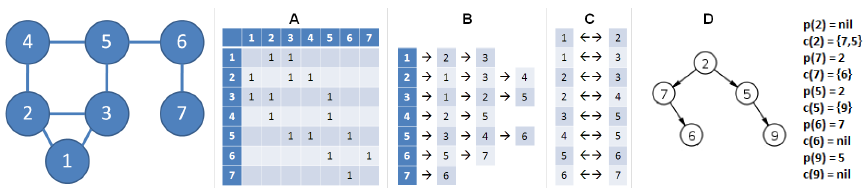
\includegraphics[width=\columnwidth]{fig/graph_representation.png}
    \caption{Four ways of graph representation, renumerate it from 0. Redraw the graph}
    \label{fig:graph_represent}
\end{figure}

\paragraph{Double Edges in Undirected Graphs} In directed graph, the number of edges is denoted as $|E|$. However, for the undirected graph, because one edge $(u, v)$ only means that vertex $u$ and $v$ are connected; we can reach to  $v$ from $u$ and it also works the other way around. To represent undirected graph, we have to double its number of edges shown in the structure; it becomes $2|E|$ in all of our representations. %From now on, for a given graph, $G = (V, E)$, for directed graph, we have $|V|$, $|E|$

\subsubsection{Adjacency Matrix}
An adjacency matrix of a graph is a 2-D matrix of size $|V|\times|V|$: each dimension, row and column, is vertex-indexed. Assume our matrix is \texttt{am}, if there is an edge between vertices 3,4, and if its unweighted graph, we mark it by setting \texttt{am[3][4]=1}, we do the same for all edges and leaving all other spots in the matrix zero-valued.  For undirected graph, it will be a symmetric matrix along the main diagonal as shown in A of Fig.~\ref{fig:graph_represent}; the matrix is its own transpose: $am = {am}^T$. We can choose to store only the entries on and above the diagonal of the matrix, thereby cutting the memory need in half.   For unweighted graph, typically our adjacency matrix is zero-and-one valued. For a weighted graph, the adjacency matrix becomes a weight matrix, with $w(i, j)$ to denote the weight of edge $(i, j)$; the weight can be both negative or positive or even zero-valued in practice, thus we might want to figure out how to distinguish the non-edge relation from the edge relation when the situation arises. 

The Python code that implements the adjacency matrix for the graph in the example is:
\begin{lstlisting}[language=Python, numbers=none]
am = [[0]*7 for _ in range(7)]

# set 8 edges
am[0][1] = am[1][0] = 1
am[0][2] = am[2][0] = 1
am[1][2] = am[2][1] = 1
am[1][3] = am[3][1] = 1
am[2][4] = am[4][2] = 1
am[3][4] = am[4][3] = 1
am[4][5] = am[5][4] = 1
am[5][6] = am[6][5] = 1
\end{lstlisting}

\paragraph{Applications} Adjacency matrix usually fits well to the dense graph where the edges are close to $|V|^2$, leaving a small ratio of the matrix be blank and unused. Checking if an edge exists between two vertices takes only $O(1)$. However, an adjacency matrix requires exactly $O(V)$ to enumerate the the neighbors of a vertex $v$--an operation commonly used in many graph algorithms--even if vertex $v$ only has a few neighbors. Moreover, when the graph is sparse, an adjacency matrix will be both inefficient in the space and iteration cost, a better option is adjacency list. %For the above example, our matrix will be:

%%%%%%%%%%%%%%%%%%%List%%%%%%%%%%
\subsubsection{Adjacency List}
An adjacency list is a more compact and space efficient form of graph representation compared with the above adjacency matrix. In adjacency list, we have a list of $V$ vertices which is vertex-indexed, and for each vertex $v$ we store anther list of neighboring nodes with their vertex  as the value, which can be represented with an array or linked list.  For example,  with adjacency list as $[[1,2,3],[3,1],[4,6,1]]$, node 0 connects to 1,2,3, node 1 connect to 3,1, node 2 connects to 4,6,1. 

In Python, We can use a normal 2-d array to represent the adjacent list, for the same graph in the example, it as represented with the following code:
\begin{lstlisting}[language=Python, numbers=none]
al = [[] for _ in range(7)]

# set 8 edges
al[0] = [1, 2]
al[1] = [2, 3]
al[2] = [0, 4]
al[3] = [1, 4]
al[4] = [2, 3, 5]
al[5] = [4, 6]
al[6] = [5]
\end{lstlisting}

\paragraph{Applications}
The upper bound space complexity for adjacency list is $O(|V|^2)$. However, with adjacency list, to check if there is an edge between node $u$ and $v$, it has to take $O(|V|)$ time complexity  with a linear scanning in the list \texttt{al[u]}. If the graph is static, meaning we do not add more vertices but can modify the current edges and its weight, we can use a set or a dictionary Python data type on second dimension of the adjacency list. This change  enables $O(1)$ search of an edge just as of in the adjacency matrix. 

%%%%%%%%%%%%%%%%%%%%%%%%Edge List%%%%%%%%%%%%%%%
\subsubsection{Edge List}
The edge list is a list of edges (one-dimensional), where the index of the list does not relate to vertex and each edge is usually in the form of (starting vertex, ending vertex, weight). We can use either a \texttt{list} or a \texttt{tuple} to represent an edge. The edge list representation of the example is given:
\begin{lstlisting}[language=Python, numbers=none]
el = []
el.extend([[0, 1], [1, 0]])
el.extend([[0, 2], [2, 0]])
el.extend([[1, 2], [2, 1]])
el.extend([[1, 3], [3, 1]])
el.extend([[3, 4], [4, 3]])
el.extend([[2, 4], [4, 2]])
el.extend([[4, 5], [5, 4]])
el.extend([[5, 6], [6, 5]])
\end{lstlisting}
\paragraph{Applications}
Edge list is not widely used as the AM and AL, and usually only be needed in a subrountine of algorithm implementation--such as in Krukal's algorithm to fine Minimum Spanning Tree(MST)--where we might need to order the edges by its weight. 

% Function to generate the list of all edges from either Adjacency Matrix or Adjacency List is similar to the following code:
% \begin{lstlisting}[language=Python]
% def generate_edges(graph):
%     edges = []
%     for node in graph:
%         for neighbour in graph[node]:
%             edges.append((node, neighbour))

%     return edges

% print(generate_edges(graph))
% \end{lstlisting}
\subsubsection{Tree Structure}
If the connected graph has no cycle and the edges $E = V-1$, which is essentially a tree. We can choose to represent it either one of the three representations. Optionally, we can use the tree structure is formed as rooted tree with \texttt{nodes} which has value and pointers to its children. We will see later how this type of tree is implemented in Python. 

\subsection{Use Dictionary}
In the last section, we always use the vertex indexed structure, it works but might not be human-friendly to work with, in practice a vertex always comes with a ``name''--such as in the cities system, a vertex should be a city's name. Another inconvenience is when we have no idea of the total number of vertices, using the index-numbering system requires us to first figure our all vertices and number each, which is an overhead. 

To avoid the two inconvenience, we can replace Adjacency list, which is a list of lists with embedded dictionary structure which is a dictionary of dictionaries or sets.   
\paragraph{Unweighted Graph}For example, we demonstrate how to give a ``name'' to exemplary graph; we replace $0$ with `a', $1$ with `b', and the others with $\{'c', d, 'e', 'f', 'g'\}$. We declare \texttt{ defaultdict(set)}, the outer list is replaced by the dictionary, and the inner neighboring node list is replaced with a \texttt{set} for $O(1)$ access to any edge.  

In the demo code, we simply construct this representation from the edge list.
\begin{lstlisting}[language=Python]
from collections import defaultdict

d = defaultdict(set)
for v1, v2 in el:
  d[chr(v1 + ord('a'))].add(chr(v2 + ord('a')))
print(d)
\end{lstlisting}
And the printed graph is as follows:
\begin{lstlisting}[numbers=none]
defaultdict(<class 'set'>, {'a': {'b', 'c'}, 'b': {'d', 'c', 'a'}, 'c': {'b', 'e', 'a'}, 'd': {'b', 'e'}, 'e': {'d', 'c', 'f'}, 'f': {'e', 'g'}, 'g': {'f'}})
\end{lstlisting}
\paragraph{Weighted Graph} If we need weights for each edge, we can use two-dimensional dictionary. We use $10$ as a weight to all edges just to demonstrate. 
\begin{lstlisting}[language=Python]
dw = defaultdict(dict)
for v1, v2 in el:
  vn1 = chr(v1 + ord('a'))
  vn2 = chr(v2 + ord('a'))
  dw[vn1][vn2] = 10
print(dw)
\end{lstlisting}
We can access the edge and its weight through \texttt{dw[v1][v2]}. The output of this structure is given:
\begin{lstlisting}[numbers=none]
defaultdict(<class 'dict'>, {'a': {'b': 10, 'c': 10}, 'b': {'a': 10, 'c': 10, 'd': 10}, 'c': {'a': 10, 'b': 10, 'e': 10}, 'd': {'b': 10, 'e': 10}, 'e': {'d': 10, 'c': 10, 'f': 10}, 'f': {'e': 10, 'g': 10}, 'g': {'f': 10}})
\end{lstlisting}






% Path: here we only need a vector to save each path.  

% \subsubsection{Implementation}
% If we implement DFS in tree, then no need a hashmap to save the visited spot. If it is in the graph, which would very necessary. 
% \begin{lstlisting}[language = Python]
% #Recursive
% def DFS(root):
%     #END Condition
%     if not root:
%         return
%     visit(root)
%     for node in root.adjacent: 
%         if not node.visited:
%             DFS(node)
% \end{lstlisting}
% \begin{lstlisting}[language = Python]
% #Iterative, implemented using a stack
% def DFS_iter():
%     root.visited = 1
%     stack = []
%     stack.append(root)
%     while stack:
%         n=stack.pop()
%         visit(n)
%         n.visited=1
%         for node in n.adjacent:
%             if not node.visited:
%                 stack.append(node)
% \end{lstlisting}



%%%%%%%%%%%%%%%%%%%%%%%Tree Representation
\section{Tree Data Structures}

In this section, we focus on implementing a \textbf{recursive} tree structure, since a free tree just works the same way as of the graph structure. Also, we have already covered the implicit structure of tree in the topic of heap. In this section, we first implement the recursive tree data structure and the construction of a tree. In the next section, we discuss the searching strategies on the tree--tree traversal, including its both recursive and iterative variants.
% A binary tree is made of nodes which has at most two branches--the ``left child" and the ``right child"--and a data element. The ``root" node is the topmost node in the tree. The left and right child recursively point to smaller ``subtrees" on either side. 


put an figure here of a binary and n-ary tree.

%\subsubsection{Nodes and Tree Construction}
Because a tree is a hierarchical--here which is represented recursively--structure of a collection of nodes. We define two classes each for the N-ary tree node and the binary tree node. A node is composed of a variable \texttt{val} saving the data and children pointers to connect the nodes in the tree.  


\paragraph{Binary Tree Node} In a binary tree, the children pointers will at at most two pointers, which we define as \texttt{left} and \texttt{right}. The binary tree node is defined as:
\begin{lstlisting}[language = Python]
class BinaryNode:
  def __init__(self, val):
    self.left = None
    self.right = None
    self.val = val
\end{lstlisting}

\paragraph{N-ary Tree Node} For N-ary node, when we initialize the length of the node's children with additional argument \texttt{n}. 
\begin{lstlisting}[language = Python]
class NaryNode:
  def __init__(self, n, val):
    self.children = [None] * n
    self.val = val
\end{lstlisting}
In this implementation, the children is ordered by each's index in the list. In real practice, there is a lot of flexibility. It is not necessarily to pre-allocate the length of its children, we can start with an empty list \texttt{[]} and just append more nodes to its children list on the fly. Also
we can replace the list with a dictionary data type, which might be a better and more space efficient way.  

\paragraph{Construct A Tree} Now that we have defined the tree node, the process of constructing a tree in the figure will be a series of operations: 
\begin{lstlisting}[numbers=none]
      1
    /   \  
   2      3
 /   \      \
4     5      6 
\end{lstlisting}
\begin{lstlisting}[language=Python]
root = BinaryNode(1)
left = BinaryNode(2)
right = BinaryNode(3)
root.left = left
root.right = right
left.left = BinaryNode(4)
left.right = BinaryNode(5)
right.right = BinaryNode(6)
\end{lstlisting}

We see that the above is not convenient in practice. A more practice way is to represent the tree with the heap-like array, which treated the tree as a complete tree. For the above binary tree, because it is not complete in definition, we pad the left child of node 3 with \texttt{None} in the list, we would have array \texttt{[1, 2, 3, 4, 5, None, 6]}. The root node will have index $0$, and given a node with index $i$, the children nodes of it will be indexed with $n*i+j, j \in [1, ..., n]$.  Thus, a better way to construct the above tree is to start from the array and and traverse the list recursively to build up the tree. 

We define a recursive function with two arguments: \texttt{a}--the input array of nodes and \texttt{idx}--indicating the position of the current node in the array. At each recursive call, we construct a \texttt{BinaryNode} and set its \texttt{left} and \texttt{right} child to be a  node returned with two recursive call of the same function. Equivalently, we can say these two subprocess--\texttt{constructTree(a, 2*idx + 1)} and \texttt{constructTree(a, 2*idx + 2)} builds up two subtrees and each is rooted with node \texttt{2*idx+1} and \texttt{2*idx+2} respectively. When there is no items left in the array to be used, it natually indicates the end of the recursive function and return \texttt{None} to indicate its an empty node. We give the following Python code:
\begin{lstlisting}[language=Python]
def constructTree(a, idx):
  '''
  a: input array of nodes
  idx: index to indicat the location of the current node
  '''
  if idx >= len(a):
    return None
  if a[idx]:
    node = BinaryNode(a[idx])
    node.left = constructTree(a, 2*idx + 1)
    node.right = constructTree(a, 2*idx + 2)
    return node
  return None
\end{lstlisting}
Now, we call this function, and pass it with out input array:
\begin{lstlisting}[language=Python]
nums = [1, 2, 3, 4, 5, None, 6]
root = constructTree(nums, 0)
\end{lstlisting}

\begin{bclogo}[couleur = blue!30, arrondi=0.1,logo=\bccrayon,ombre=true]{Please write a recursive function to construct the N-ary tree given in Fig.~\ref{}?} 
\end{bclogo}
In the next section, we discuss tree traversal methods, and we will use those methods to print out the tree we just build. 


% \section{Time complexity of Binary Tree}
% If we spent O(n) to convert $T(n)$ to $2T(n/2)$. We have the following deduction:
% \begin{equation} \label{bt_time}
% \begin{split}
% T(n) & = 2T(n/2) + O(n)\\
%  & = 2 * 2T(n/4) + O(n) + O(n)\\
%  & = O(nlogn)
% \end{split}
% \end{equation}
% which is the same  as merge sort. If the divide cost is only $O(1)$.
% \begin{equation}\label{bt_time2}
% \begin{split}
% T(n) &= 2T(n/2) + O(1)\\
% & = 2 * 2T(n/4) + O(1) + O(1)\\
% &= n + (1 + 2 + 4 +...+ n)\\
% &\approx n + 2n\\
% &\approx O(n)
% \end{split}
% \end{equation}

\subsection{LeetCode Problems}

To show the nodes at each level, we use LevelOrder function to print out the tree:
\begin{lstlisting}[language=Python]
def LevelOrder(root):
    q = [root]
    while q:
        new_q = []
        for n in q:
            if n is not None:
                print(n.val, end=',')
            if n.left:
                new_q.append(n.left)
            if n.right:
                new_q.append(n.right)
        q = new_q
        print('\n')
LevelOrder(root)
# output
# 1,

# 2,3,

# 4,5,None,6,
\end{lstlisting}
\textbf{Lowest Common Ancestor}. The lowest common ancestor is defined between two nodes p and q as the lowest node in T that has both p and q as descendants (where we allow a node to be a descendant of itself). There will be two cases in LCA problem which will be demonstrated in the following example. 
\begin{examples}[resume]
\item \textbf{Lowest Common Ancestor of a Binary Tree (L236).}  Given a binary tree, find the lowest common ancestor (LCA) of two given nodes in the tree. Given the following binary tree:  root = [3,5,1,6,2,0,8,null,null,7,4]
\begin{lstlisting}[numbers=none]
        _______3______
       /              \
    ___5__          ___1__
   /      \        /      \
   6      _2       0       8
         /  \
         7   4

Example 1:
Input: root = [3,5,1,6,2,0,8,null,null,7,4], p = 5, q = 1
Output: 3
Explanation: The LCA of of nodes 5 and 1 is 3.

Example 2:
Input: root = [3,5,1,6,2,0,8,null,null,7,4], p = 5, q = 4
Output: 5
Explanation: The LCA of nodes 5 and 4 is 5, since a node can be a descendant of itself
             according to the LCA definition.
\end{lstlisting}
\textbf{Solution: Divide and Conquer}. There are two cases for LCA: 1) two nodes each found in different subtree, like example 1. 2) two nodes are in the same subtree like example 2. If we compare the current node with the p and q, if it equals to any of them, return current node in the tree traversal. Therefore in example 1, at node 3, the left return as node 5, and the right return as node 1, thus node 3 is the LCA. In example 2, at node 5, it returns 5, thus for node 3, the right tree would have None as return, thus it makes the only valid return as the final LCA. The time complexity is $O(n)$.
\begin{lstlisting}[language=Python]
def lowestCommonAncestor(self, root, p, q):
    """
    :type root: TreeNode
    :type p: TreeNode
    :type q: TreeNode
    :rtype: TreeNode
    """
    if not root:
        return None
    if root == p or root == q:
        return root # found one valid node (case 1: stop at 5, 1, case 2:stop at 5)
    left = self.lowestCommonAncestor(root.left, p, q)
    right = self.lowestCommonAncestor(root.right, p, q)
    if left is not None and right is not None: # p, q in the subtree
        return root 
    if any([left, right]) is not None:
        return left if left is not None else right
    return None
\end{lstlisting}
\end{examples}
%%%%%%%%%%%%%%%%%%%%%%Heap and priority queue
%%%%%%%%%%%%%%%%%%Basic Implementation%%%%%%%%%%%%%%%%%%%%%%%%
%%%%%%%%%%%%%%%%%heap%%%%%%%%%%%%%%%%%
%%%%%%%%%%%%%%%%%heap%%%%%%%%%%%%%%%%%
\section{Heap}
    count = Counter(nums)
%%%%%%%%%%%%%%%%%%%%%%%%%%%%%%%%%%%%%%%
% In this section, we introduce heap data structures which is essentially an array object but it can be viewed as a nearly complete binary tree. The concept of the data structures in this chapter is between liner and non-linear, that is using linear data structures to mimic the non-linear data structures and its behavior for higher efficiency under certain context. 

Heap is a tree based data structure that satisfies \textit{the heap ordering property}. The ordering can be one of two types:
\begin{itemize}
    \item the min-heap property: the value of each node is greater than or equal ($\geq$) to the value of its parent, with the minimum-value element at the root.
\item the max-heap property: the value of each node is less than or equal to ($\leq$) the value of its parent, with the maximum-value element at the root. 
\end{itemize}
\paragraph{Binary Heap}
\begin{figure}[h!]
    \centering
    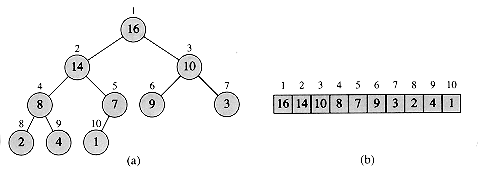
\includegraphics[width = 0.98\columnwidth]{fig/binary_tree.png}
    \caption{Max-heap be visualized with binary tree structure on the left, and be implemented with Array on the right.}
    \label{fig:max-heap-1}
\end{figure}
A heap is not a sorted structure but can be regarded as partially ordered. The maximum number of children of a node in a heap depends on the type of heap. However, in the more commonly-used heap type, there are at most two children of a node and it's known as a Binary heap. A min-binary heap is shown in Fig.~\ref{fig:max-heap-1}. Throughout this section the word ``heap'' will always refer to a min-heap. 

Heap is commonly used to implement priority queue that each time the item of the highest priority is popped out -- this can be done in $O(\log n)$. As we go through the book, we will find how often priority queue is needed to solve our problems.  It can also be used in sorting, such as the heapsort algorithm. 

\paragraph{Heap Representation}
A binary heap is always a complete binary tree that each level is fully filled before starting to fill the next level. Therefore it has a height of $\log n$ given a binary heap with $n$ nodes.  A complete binary tree can be uniquely represented by storing its level order traversal in an array.  Array representation more space efficient  due to the non-existence of the children pointers for each node. 

In the array representation, index 0 is skipped for convenience of implementation. Therefore, root locates at index 1. Consider a k-th item of the array, its parent and children relation is:
\begin{itemize}
    \item its left child is located at $2*k$ index, 
    \item its right child is located at $2*k+1$. index, 
    \item and its parent is located at $k/2$ index (In Python3, use integer division $n//2$).
\end{itemize}


% In Python3, use integer division $n//2$. \textit{Note: we can start index with 0 as used in \textbf{heapq} library introduced later in this section. Given a node $x$, the left and right child will be $2*x+1$, $2*x+2$, and the parent node will have index $(x-1)//2$.}


% Normally, there is usually no notion of 'search' in heap, but only insertion and deletion, which can be done by traversing a $O(\log n)$ leaf-to-root or root-to-leaf path. 


\subsection{Basic Implementation}
The basic methods of a heap class should include: \texttt{push}--push an item into the heap, \texttt{pop}--pop out the first item, and \texttt{heapify}--convert an arbitrary array into a heap. In this section, we use the heap shown in Fig.~\ref{fig:min-heap} as our example. 
\begin{figure}[h!]
    \centering
    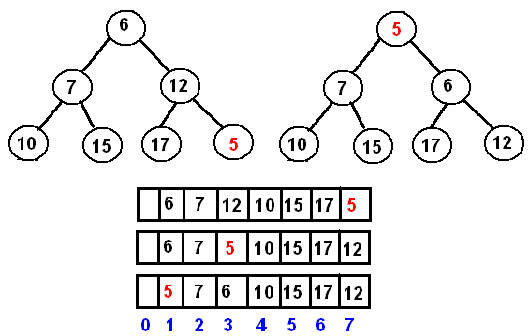
\includegraphics[width = 0.8\columnwidth]{fig/min_heap_push.png}
    \caption{A Min-heap.}
    \label{fig:min-heap}
\end{figure}
\paragraph{Push:  Percolation Up} The new element is initially appended to the end of the heap (as the last element of the array). The heap property is repaired by comparing the added element with its parent and moving the added element up a level (swapping positions with the parent). This process is called \textit{percolation up}. The comparison is repeated until the parent is larger than or equal to the percolating element.  When we push an item in,  the item is initially appended to the end of the heap. Assume the new item  is the smaller than existing items in the heap, such as $5$ in our example, there will be violation of the heap property through the path from the end of the heap to the root.  To repair the violation,  we traverse through the path and compare the added item with its parent: 
\begin{itemize}
    \item if parent is smaller than the added item, no action needed and the traversal is terminated, e.g. adding item 18 will lead to no action. 
    \item otherwise, swap the item with the parent, and set the node to its parent so that it can keep traverse. 
\end{itemize}
Each step we fix the heap ordering property for a substree. 
 The time complexity is the same as the height of the complete tree, which is $O(\log n)$. 
 
 To generalize the process, a \texttt{\_float()} function is first implemented which enforce min heap ordering property on the path from a given index to the root. 
\begin{lstlisting}[language=Python]
def _float(idx, heap): 
  while idx // 2: 
      p = idx // 2
      # Violation
      if heap[idx] < heap[p]:
          heap[idx], heap[p] = heap[p], heap[idx]
      else:
        break
      idx = p 
  return
\end{lstlisting}
With  \texttt{\_float()}, function \texttt{push} is implemented as:
\begin{lstlisting}[language=Python]
def push(heap, k):
  heap.append(k)
  _float(idx = len(heap) - 1, heap=heap)
\end{lstlisting}

\paragraph{Pop: Percolation Down} When we pop out the item, no matter if it is the root item or any other item in the heap, an empty spot appears at that location. We first move the last item in the heap to this spot, and then start to repair the heap ordering property by comparing the new item at this spot to its children: 
\begin{itemize}
    \item if one of its children has smaller value than this item, swap this item with that child and set the location to that child's location. And then continue.
    \item otherwise, the process is done.
\end{itemize} 
\begin{figure}[h!]
    \centering
    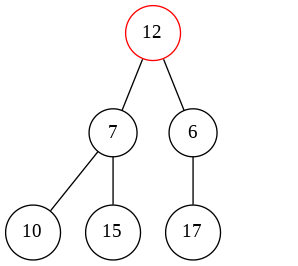
\includegraphics[width = 0.44\columnwidth]{fig/min_heap_insert.png}
    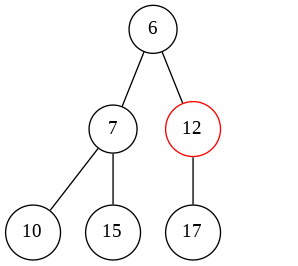
\includegraphics[width = 0.44\columnwidth]{fig/min_heap_insert_step1.png}
        \caption{Left: delete node 5, and move node 12 to root. Right: 6 is the smallest among 12, 6, and 7, swap node 6 with node 12.}
    \label{fig:min-heap-pop}
\end{figure}
Similarly, this process is called \textit{percolation down}. Same as the insert in the case of complexity, $O(\log n)$. We demonstrate this process with two cases:
\begin{itemize}
    \item if the item is the root, which is the minimum item $5$ in our min-heap example,  we move 12 to the root first. Then we compare 12 with its two children, which are 6 and 7. Swap 12 with 6, and continue. The process is shown in Fig.~\ref{fig:min-heap-pop}.
    \item if the item is any other node instead of root, say node 7 in our example. The process is exactly the same. We move 12 to node 7's position. By comparing 12 with children 10 and 15, 10 and 12 is about to be swapped. With this, the heap ordering property is sustained. 
\end{itemize}

We first use a function \texttt{\_sink} to implement the percolation down part of the operation. 
\begin{lstlisting}[language=Python]
def _sink(idx, heap): 
  size = len(heap)
  while 2 * idx < size:
    li = 2 * idx
    ri = li + 1
    mi = idx
    if heap[li] < heap[mi]:
      mi = li
    if ri < size and heap[ri] < heap[mi]:
      mi = ri
    if mi != idx:
        # swap index with mi
        heap[idx], heap[mi] = heap[mi], heap[idx]
    else:
      break
    idx = mi
\end{lstlisting}
The \texttt{pop} is implemented as:
\begin{lstlisting}[language=Python]
def pop(heap):
    val = heap[1]
    # Move the last item into the root position
    heap[1] = heap.pop()
    _sink(idx=1, heap=heap)
    return val
\end{lstlisting}


\paragraph{Heapify}  Heapify is a procedure that converts a list to a heap.  To heapify a list, we can naively do it through a series of insertion operations through the items in the list, which gives us an upper-bound time complexity : $O(n\log n)$. However, a more efficient way is to treat the given list as a tree and to heapify directly on the list. %There are two possibly two ways to do this: (1) through sinking and (2) through floating.  

To satisfy the heap property, we need to first start from the smallest subtrees, which are leaf nodes. Leaf nodes  have no children which satisfy the heap property naturally. Therefore we can jumpy to the last parent node, which is at position \texttt{n//2} with starting at 1 index. We apply the percolation down process as used in \texttt{pop}  operation which works forwards comparing the node with its children nodes and applies swapping if the heap property is violated. At the end, the subtree rooted at this particular node obeys the heap ordering property. We then repeat the same process for all parents nodes items in the list in range $[n/2, 1]$--in reversed order of $[1, n/2]$, which guarantees that the final complete binary tree is a binary heap. This follows a dynamic programming fashion.  The leaf nodes $a[n/2+1, n]$ are naturally a heap. Then the subarrays are heapified in order of  $a[n/2, n]$, $a[n/2-1, n], ..., [1, n]$ as we working on nodes $[n/2, 1]$.  we first heaipfy $a[n, n], A[n-1...n], A[n-2...n], ..., A[1...n]$.  Such process gives us a tighter upper bound which is $O(n)$. 

We show how the heapify process is applied on $a=[21, 1, 45, 78, 3, 5]$ in Fig.~\ref{fig:heapify}.  
% \begin{figure}[h!]
%     \centering
%     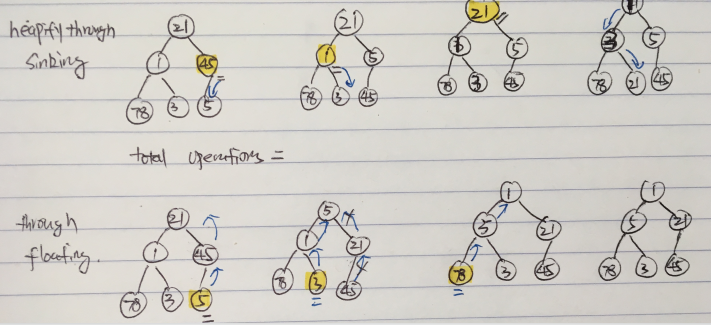
\includegraphics[width = 0.98\columnwidth]{fig/heapify.png}
%     \caption{Heapify for a given list.}
%     \label{fig:heapify}
% \end{figure}
\begin{figure}[h!]
    \centering
    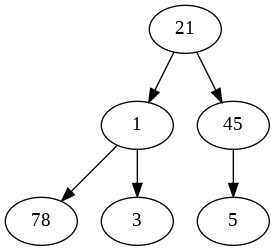
\includegraphics[width = 0.3\columnwidth]{fig/min_heap_heapify_1.png}
    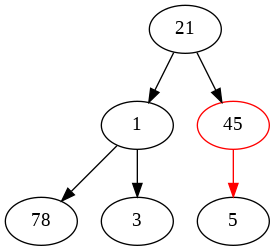
\includegraphics[width = 0.3\columnwidth]{fig/min_heap_heapify_2.png}
    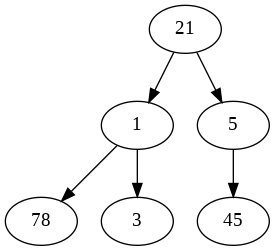
\includegraphics[width = 0.3\columnwidth]{fig/min_heap_heapify_3.png}
    \caption{Heapify: The last parent node 45.}
    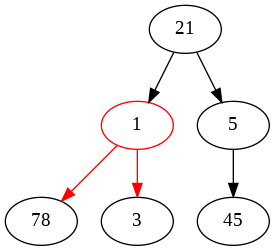
\includegraphics[width = 0.3\columnwidth]{fig/min_heap_heapify_4.png}
    \caption{Heapify: On node 1}
    
    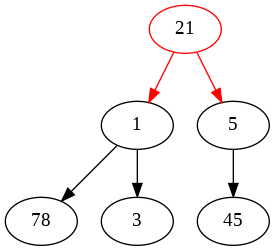
\includegraphics[width = 0.3\columnwidth]{fig/min_heap_heapify_5.png}
    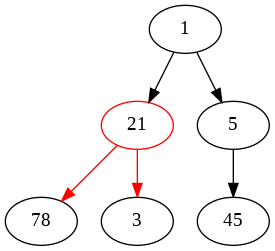
\includegraphics[width = 0.3\columnwidth]{fig/min_heap_heapify_6.png}
    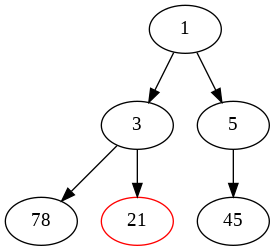
\includegraphics[width = 0.3\columnwidth]{fig/min_heap_heapify_7.png}
    \caption{Heapify: On node 21.}
    \label{fig:heapify}
\end{figure}

Implementation-wise, the \texttt{heapify} function call \texttt{\_sink} as its subroutine. The code is shown as:
\begin{lstlisting}[language=Python]
def heapify(lst):
    heap = [None] + lst
    n = len(lst)
    for i in range(n//2, 0, -1):
      _sink(i, heap)
    return heap
\end{lstlisting}

% Now, run the following code:
% \begin{lstlisting}[language=Python]
% h = Heap()
% h.heapify(lst)
% print('heapify with heapify:', h)
% \end{lstlisting}
% Out put is:
% \begin{lstlisting}
% heapify with heapify: 1 5 21 78 3 45 
% \end{lstlisting}
\begin{bclogo}[couleur = blue!30, arrondi=0.1,logo=\bccrayon,ombre=true]{Which way is more efficient building a heap from a list?} Using insertion or heapify? What is the efficiency of each method? The experimental result can be seen in the code.
\end{bclogo}

\begin{bclogo}[couleur = blue!30, arrondi=0.1,logo=\bccrayon,ombre=true]{Try to use the percolation up process to heaipify the list. } 
\end{bclogo}

% \begin{enumerate}
% \item MAX-HEAPIFY, runs in $O(lgn)$, is the key to maintaining the max-heap property
% \item BUILD-MAX-HEAP, runs in linear time, produces a maxheap from an unordered input array
% \item MAX-HEAP-INSERT, HEAP-EXTRACT-MAX, HEAP-INCREASE-KEY, and HEAP-MAXIMUM, runs in $O(lgn)$ time, allow the heap data structure to implement a priority queue
% \end{enumerate}
%%%%%%%%%%%%%%%%%%Python Built-in Module: heapq%%%%%%%%%%%%%%%%%%%%%%%%
\subsection{Python Built-in Library: \texttt{heapq}}
When we are solving a problem, unless specifically required for implementation, we can always use an existent Python module/package. \texttt{heapq} is one of the most frequently used library in problem solving. 

\texttt{heapq}~\footnote{\url{https://docs.python.org/3.0/library/heapq.html}} is a built-in library in Python that implements heap queue algorithm. \texttt{heapq} object implements a minimum binary heap  and it provides three main functions: \texttt{heappush}, \texttt{heappop}, and \texttt{heaipfy} similar to what we have implemented in the last section. The API differs from our last section in one aspect: it uses zero-based indexing. There are other three functions: \texttt{nlargest}, \texttt{nsmallest}, and \texttt{merge} that come in handy in practice. These functions are listed and described in Table~\ref{tab:functions_in_heapq}.% \textit{To note that heapq is not a data type like queue.Queue() or collections.deque(), it is a library (or class) that can do operations like it is on a heap.} %, which can be used to maintain a priority queue. Operations include heappush, heappop, and nsmallest. heapq in python to maintain a priority queue with $O(logn)$.
\begin{table}[h]
\begin{small}
\centering
\noindent\captionof{table}{ Methods of \textbf{heapq}}
 \noindent \begin{tabular}{|p{0.25\columnwidth}|p{0.75\columnwidth}| }
  \hline
Method & Description   \\ \hline
{heappush(h, x)}  &  Push the \texttt{x} onto the heap, maintaining the heap invariant.  \\\hline
{heappop(h)}  &Pop and return the \textit{smallest} item from the heap, maintaining the heap invariant. If the heap is empty, \texttt{IndexError} is raised.\\ \hline
{heappushpop(h, x)}  &Push \texttt{x} on the heap, then pop and return the smallest item from the heap. The combined action runs more efficiently than {heappush()} followed by a separate call to \texttt{heappop()}.\\ \hline
{heapify(x)} & Transform list \texttt{x} into a heap, in-place, in linear time.\\ \hline
{nlargest(k, iterable, key = fun)} & This function is used to return the \texttt{k} largest elements from the iterable specified and satisfying the key if mentioned. \\ \hline
{nsmallest(k, iterable, key = fun)} & This function is used to return the \texttt{k} smallest elements from the iterable specified and satisfying the key if mentioned. \\ \hline

{merge(*iterables, key=None, reverse=False)} & Merge multiple sorted inputs into a single sorted output. Returns a \textit{generator} over the sorted values. \\ \hline
{heapreplace(h, x)} & Pop and return the smallest item from the heap, and also push the new item.\\ \hline
\end{tabular}
  \label{tab:functions_in_heapq}
  \end{small}
\end{table} 

Now, lets see some examples. 
\paragraph{Min-Heap} Given the exemplary list $a =[21, 1, 45, 78, 3, 5]$, we call the function \texttt{heapify()} to convert it to a min-heap. 
\begin{lstlisting}[language = Python]
from heapq import heappush, heappop, heapify
h = [21, 1, 45, 78, 3, 5]
heapify(h)
\end{lstlisting}
The heapified result is $h=[1, 3, 5, 78, 21, 45]$. Let's try \texttt{heappop} and \texttt{heappush}:
\begin{lstlisting}[language=Python]
heappop(h)
heappush(h, 15)
\end{lstlisting}
The print out for \texttt{h} is:
\begin{lstlisting}[language=Python]
[5, 15, 45, 78, 21]
\end{lstlisting}

\paragraph{\texttt{nlargest} and \texttt{nsmallest}}
To get the largest or smallest first $n$ items with these two functions does not require the list to be first heapified with \texttt{heapify} because it is built in them.
\begin{lstlisting}[language=Python]
from heapq import nlargest, nsmallest
h = [21, 1, 45, 78, 3, 5]
nl = nlargest(3, h)
ns = nsmallest(3, h)
\end{lstlisting}
The print out for \texttt{nl} and \texttt{ns} is as:
\begin{lstlisting}
[78, 45, 21]
[1, 3, 5]
\end{lstlisting}

\paragraph{Merge Multiple Sorted Arrays}  Function \texttt{merge} merges multiple iterables into a single generator typed output. It assumes all the inputs are sorted. For example:
\begin{lstlisting}[language=Python]
from heapq import merge
a = [1, 3, 5, 21, 45, 78]
b = [2, 4, 8, 16]
ab = merge(a, b)
\end{lstlisting}
The print out of $ab$ directly can only give us a generator object with its address in the memory:
\begin{lstlisting}[language=Python]
<generator object merge at 0x7fdc93b389e8>
\end{lstlisting}
We can use list comprehension and iterate through $ab$ to save the sorted array in a list:
\begin{lstlisting}[language=Python]
ab_lst = [n for n in ab]
\end{lstlisting}
The print out for \texttt{ab\_lst} is:
\begin{lstlisting}[language=Python]
[1, 2, 3, 4, 5, 8, 16, 21, 45, 78]
\end{lstlisting}


\paragraph{Max-Heap} As we can see the default heap implemented in  \texttt{heapq}  is forcing the heap property of the min-heap. What if we want a max-heap instead? In the library, it does offer us function, but it is intentionally hided from users. It can be accessed like: \texttt{heapq.\_[function]\_max()}. Now, we can heapify a max-heap with function \texttt{\_heapify\_max}.
\begin{lstlisting}[language = Python]
from heapq import _heapify_max
h = [21, 1, 45, 78, 3, 5]
_heapify_max(h)
\end{lstlisting}
The print out for \texttt{h} is:
\begin{lstlisting}
[78, 21, 45, 1, 3, 5]
\end{lstlisting}

Also, in practise, a simple hack for the max-heap is to save data as negative. Whenever we use the data, we convert it to the original value. For example: 
\begin{lstlisting}[language=Python]
h = [21, 1, 45, 78, 3, 5]
h = [-n for n in h]
heapify(h)
a = -heappop(h)
\end{lstlisting}
\texttt{a} will be 78, as the largest item in the heap. 

% \paragraph{More Private Functions}
% \begin{table}[h]
% \begin{small}
% \centering
% \noindent\captionof{table}{ Private Methods of \textbf{heapq}}
%  \noindent \begin{tabular}{|p{0.25\columnwidth}|p{0.75\columnwidth}| }
%   \hline
% Method & Description   \\ \hline
% heappush(h, x)  &  Push the value item onto the heap, maintaining the heap invariant.  \\\hline
% heappop(h)  &Pop and return the \textit{smallest} item from the heap, maintaining the heap invariant. If the heap is empty, IndexError is raised.\\ \hline
% heappushpop(h, x)  &Push item on the heap, then pop and return the smallest item from the heap. The combined action runs more efficiently than heappush() followed by a separate call to heappop().\\ \hline
% heapify(x) & Transform list x into a heap, in-place, in linear time.\\ \hline
% heapreplace(h, x) & Pop and return the smallest item from the heap, and also push the new item. The heap size doesn’t change. If the heap is empty, IndexError is raised. This is more efficient than heappop() followed by heappush(), and can be more appropriate when using a fixed-size heap.\\ \hline
% nlargest(k, iterable, key = fun) & This function is used to return the k largest elements from the iterable specified and satisfying the key if mentioned. \\ \hline
% nsmallest(k, iterable, key = fun) & This function is used to return the k smallest elements from the iterable specified and satisfying the key if mentioned. \\ \hline
% \end{tabular}
%   \label{tab:functions_in_heapq}
%   \end{small}
% \end{table} 

\paragraph{With Tuple/List or Customized Object as Items for Heap}
Any object that supports comparison (\texttt{\_cmp\_()}) can be used in heap with \texttt{heapq}. When we want our item to include information such as ``priority'' and ``task'', we can either put it in a tuple or a list. \texttt{heapq} For example, our item is a list, and the first is the priority and the second denotes the task id.
\begin{lstlisting}
heap = [[3, 'a'], [10, 'b'], [5,'c'], [8, 'd']]
heapify(heap)
\end{lstlisting}
The print out for \texttt{heap} is:
\begin{lstlisting}[language=Python]
[[3, 'a'], [8, 'd'], [5, 'c'], [10, 'b']]
\end{lstlisting}
However, if we have multiple tasks that having the same priority, the relative order of these tied tasks can not be sustained. This is because the list items are compared with the whole list as key: it first compare the first item, whenever there is a tie, it compares the next item. For example, when our example has multiple items with $3$ as the first value in the list. 
\begin{lstlisting}[language=Python]
h = [[3, 'e'], [3, 'd'], [10, 'c'], [5,'b'], [3, 'a']]
heapify(h)
\end{lstlisting}
The printout indicates that the relative ordering of items [3, 'e'], [3, 'd'], [3, 'a'] is not kept:
\begin{lstlisting}[language=Python]
[[3, 'a'], [3, 'd'], [10, 'c'], [5, 'b'], [3, 'e']]
\end{lstlisting}
Keeping the relative order of tasks with same priority is a requirement for \textit{priority queue} abstract data structure. We will see at the next section how priority queue can be implemented with \texttt{heapq}. 

\paragraph{Modify Items in \texttt{heapq}}
In the heap, we can change the value of any item just as what we can in the list. However, the violation of heap ordering property occurs after the change so that we need a way to fix it. We have the following two private functions to use according to the case of change: 
\begin{itemize}
    \item\texttt{\_siftdown(heap, startpos, pos)}: \texttt{pos} is where the where the new violation is. \texttt{startpos} is till where we want to restore the heap invariant, which is usually set to $0$. Because in \texttt{\_siftdown()} it goes backwards to compare this node with the parents, we can call this function to fix when an item's value is decreased. 
    \item \texttt{\_siftup(heap, pos)}: In \texttt{\_siftup()} items starting from \texttt{pos} are compared with their children so that smaller items are sifted up along the way. Thus, we can call this function to fix when an item's value is increased. 
\end{itemize}
We show one example:
\begin{lstlisting}[language=Python]
import heapq
heap = [[3, 'a'], [10, 'b'], [5,'c'], [8, 'd']]
heapify(heap)
print(heap)

heap[0] = [6, 'a']
# Increased value
heapq._siftup(heap, 0) 
print(heap)
#Decreased Value
heap[2] = [3, 'a']
heapq._siftdown(heap, 0, 2)
print(heap)
\end{lstlisting}
The printout is:
\begin{lstlisting}[language=Python]
[[3, 'a'], [8, 'd'], [5, 'c'], [10, 'b']]
[[5, 'c'], [8, 'd'], [6, 'a'], [10, 'b']]
[[3, 'a'], [8, 'd'], [5, 'c'], [10, 'b']]
\end{lstlisting}

%%%%%%%%%%%%%%%%%%%%priority Queue%%%%%%%%%%%%%%%%%%%
\section{Priority Queue}
\label{sec_priority_queue}
A priority queue is an abstract data type(ADT) and an extension of queue with properties: 
\begin{enumerate}
    \item A queue that each item has a priority associated with.
    \item In a priority queue, an item with higher priority is served (dequeued) before an item with lower priority. 
    \item If two items have the same priority, they are served according to their order in the queue. 
\end{enumerate}
Priority Queue is commonly seen applied in:
\begin{enumerate}
    \item CPU Scheduling, 
    \item Graph algorithms like Dijkstra’s shortest path algorithm, Prim’s Minimum Spanning Tree, etc.
    \item All queue applications where priority is involved. 
\end{enumerate}
The  properties of priority queue demand sorting stability to our chosen sorting mechanism or data structure.  Heap is generally preferred over arrays or linked list to be the underlying data structure for priority queue. In fact, the Python class  \texttt{PriorityQueue()} from Python module \texttt{queue} uses \texttt{heapq} under the hood too. 
We later will see how to implement priority queue with \texttt{heapq} and how to use \texttt{PriorityQueue()} class for our purpose. In default, the lower the value is, the higher the priority is, making min-heap the underlying data structure. 
\subsubsection{Implement with \texttt{heapq}  Library} 

The core functions: \texttt{heapify()}, \texttt{push()}, and \texttt{pop()} within \texttt{heapq} lib are used in our implementation. In order to implement priority queue, our binary heap needs to have the following features:
\begin{itemize}
    \item \textbf{Sort stability:} when we get two tasks with equal priorities, we return them in the same order as they were originally added. A potential solution is to modify the original 2-element list \texttt{[priority, task]} into a 3-element list as \texttt{[priority, count, task]}. \texttt{list} is preferred because \texttt{tuple} does not allow item assignment. The entry \texttt{count} indicates the original order of the task in the list, which serves as a tie-breaker so that two tasks with the same priority are returned in the same order as they were added to preserve the sort stability. Also, since no two entry counts are the same so that in the tuple comparison  the task will never be directly compared with the other. For example, use the same example as in the last section:
\begin{lstlisting}[language=Python]
import itertools
counter = itertools.count()
h = [[3, 'e'], [3, 'd'], [10, 'c'], [5,'b'], [3, 'a']]
h = [[p, next(counter), t] for p, t in h]
\end{lstlisting}
The printout for \texttt{h} is:
\begin{lstlisting}[language=Python]
[[3, 0, 'e'], [3, 1, 'd'], [10, 2, 'c'], [5, 3, 'b'], [3, 4, 'a']]
\end{lstlisting}
If we \texttt{heapify} \texttt{h} will gives us the same order as the original \texttt{h}. The relative ordering of ties in the sense of priority is sustained. 
\item \textbf{Remove arbitrary items or update the priority of an item:} In situations such as the priority of a task changes or if a pending task needs to be removed, we have to update or remove an item from the heap. we have seen how to update an item's value in $O(\log n)$ time cost with two functions: \texttt{\_siftdown()} and \texttt{\_siftup()} in a heap. However, how to remove an arbitrary item? We could have found and replaced it with the last item in the heap. Then depending on the comparison between the value of the deleted item and the last item, the two mentioned functions can be applied further. 

However, there is a more convenient alternative: whenever we ``remove'' an item, we do not actually remove it but instead simply mark it as ``removed''. These ``removed'' items will eventually be popped out through a normally \texttt{pop} operation that comes with heap data structure, and which has the same time cost $O(\log n)$. With this alternative, when we are updating an item, we mark the old item as ``removed'' and add the new item in the heap. Therefore, with the special mark method, we are able to implement a heap wherein arbitrary removal and update is supported with just three common functionalities: \texttt{heapify}, \texttt{heappush}, and \texttt{heappop}. 

Let's use the same example here. We first remove task `d' and then update task `b''s priority to 14. Then we use another list \texttt{vh} to get the relative ordering of tasks in the heap according to the priority.
\begin{lstlisting}[language=Python]
REMOVED = '<removed-task>'
# Remove task 'd'
h[1][2] = REMOVED
# Updata task 'b''s proprity to 14
h[3][2] = REMOVED
heappush(h, [14, next(counter), 'b'])
vh = []
while h:
  item = heappop(h)
  if item[2] != REMOVED:
    vh.append(item)
\end{lstlisting}
The printout for \texttt{vh} is:
\begin{lstlisting}[language=Python]
[[3, 0, 'e'], [3, 4, 'a'], [10, 2, 'c'], [14, 5, 'b']]
\end{lstlisting}

\item \textbf{Search in constant time:} To search in the heap of an arbitrary item--non-root item and root-item--takes linear time. In practice, tasks should have unique task ids to distinguish from each other, making the usage of a  \texttt{dictionary} where \texttt{task} serves as key and the the 3-element list as value possible (for a list, the value is just a pointer pointing to the starting position of the list). With the dictionary to help search, the time cost is thus decreased to constant. We name this dictionary here as \texttt{entry\_finder}. Now, with we modify the previous code. The following code shows how  to add items into a heap that associates with \texttt{entry\_finder}:
\begin{lstlisting}[language=Python]
# A heap associated with entry_finder
counter = itertools.count()
entry_finder = {}
h = [[3, 'e'], [3, 'd'], [10, 'c'], [5,'b'], [3, 'a']]
heap = []
for p, t in h:
  item = [p, next(counter), t]
  heap.append(item)
  entry_finder[t] = item
heapify(heap)
\end{lstlisting}
Then, we execute the remove and update operations with \texttt{entry\_finder}. 
\begin{lstlisting}[language=Python]
REMOVED = '<removed-task>'
def remove_task(task_id):
  if task_id in entry_finder:
    entry_finder[task_id][2] = REMOVED
    entry_finder.pop(task_id) # delete from the dictionary
  return

# Remove task 'd'
remove_task('d')
# Updata task 'b''s priority to 14
remove_task('b')
new_item = [14, next(counter), 'b']
heappush(heap, new_item)
entry_finder['b'] = new_item
\end{lstlisting}
\end{itemize}
In the notebook, we provide a comprehensive class named \texttt{PriorityQueue} that implements just what we have discussed in this section.

\subsubsection{Implement with \texttt{PriorityQueue} class} Class \texttt{PriorityQueue()} class has the same member functions as class \texttt{Queue()} and \texttt{LifoQueue()} which are shown in Table~\ref{tab:methods_of_queue}. Therefore, we skip the introduction. First, we built a queue with:
\begin{lstlisting}[language=Python]
from queue import PriorityQueue
data = [[3, 'e'], [3, 'd'], [10, 'c'], [5,'b'], [3, 'a']]
pq = PriorityQueue()
for d in data:
  pq.put(d)
  
process_order = []
while not pq.empty():
  process_order.append(pq.get())
\end{lstlisting}
The printout for \texttt{process\_order} shown as follows indicates how \texttt{PriorityQueue} works the same as our \texttt{heapq}:
\begin{lstlisting}
[[3, 'a'], [3, 'd'], [3, 'e'], [5, 'b'], [10, 'c']]
\end{lstlisting}
\paragraph{Customized Object} If we want the higher the value is the higher priority, we demonstrate how to do so with a customized object with two comparison operators: \texttt{<} and \texttt{==} in the class with magic functions \texttt{\_\_lt\_\_()} and \texttt{\_\_eq\_\_()}. The code is as:
\begin{lstlisting}[language = Python]
class Job():
    def __init__(self, priority, task):
        self.priority = priority
        self.task = task
        return

    def __lt__(self, other):
        try:
            return self.priority > other.priority
        except AttributeError:
            return NotImplemented
    def __eq__(self, other): 
        try:
            return self.priority == other.priority
        except AttributeError:
            return NotImplemented
\end{lstlisting}

Similarly, if we apply the wrapper shown in the second of heapq, we can have a priority queue that is having sort stability, remove and update item, and with constant serach time. 
\begin{bclogo}[couleur = blue!30, arrondi=0.1,logo=\bccrayon,ombre=true]{In single thread programming, is \textbf{heapq} or \textbf{PriorityQueue} more efficient?} In fact, the PriorityQueue implementation uses heapq under the hood to do all prioritisation work, with the base Queue class providing the locking to make it thread-safe. While heapq module offers no locking, and operates on standard list objects. This makes the heapq module faster; there is no locking overhead. In addition, you are free to use the various heapq functions in different, noval ways, while the PriorityQueue only offers the straight-up queueing functionality. 
\end{bclogo}
\subsubsection{Hands-on Example}
\paragraph{Top K Frequent Elements (L347, medium)} Given a non-empty array of integers, return the k most frequent elements.
\begin{lstlisting}[numbers=none]
Example 1:
Input: nums = [1,1,1,2,2,3], k = 2
Output: [1,2]

Example 2:
Input: nums = [1], k = 1
Output: [1]
\end{lstlisting}

\paragraph{Analysis:} We first using a hashmap to get information as: item and its frequency. Then, the problem becomes obtaining the top k most frequent items in our counter: we can either use sorting or use heap. Our exemplary code here is for the purpose of getting familiar with related Python modules.
\begin{itemize}
    \item \textbf{Counter().} \texttt{Counter()} has function \texttt{most\_common(k)} that will return the top $k$ most frequent items. The time complexity is $O(n \log n)$. 
\begin{lstlisting}[language=Python]
from collections import Counter
def topKFrequent(nums, k):
    return [x for x, _ in Counter(nums).most_common(k)]
\end{lstlisting}

\item \textbf{\texttt{heapq.nlargest()}}. The complexity should be better than $O(n \log n)$. 
\begin{lstlisting}[language=Python]
from collections import Counter
import heapq
def topKFrequent(nums, k):
    count = collections.Counter(nums) 
    # Use the value to compare with
    return heapq.nlargest(k, count.keys(), key=lambda x: count[x]) 
\end{lstlisting}
\texttt{key=lambda x: count[x]} can also be replaced with \texttt{key=lambda x: count[x]}.

\item \textbf{PriorityQueue():} We put the negative count into the priority queue so that it can perform as a max-heap. 
\begin{lstlisting}[language=Python]
from  queue  import  PriorityQueue
def topKFrequent(self, nums, k):
    count = Counter(nums)
    pq = PriorityQueue()
    for key, c in count.items():
        pq.put((-c, key))
    return [pq.get()[1] for i in range(k)]
\end{lstlisting}
\end{itemize}
\section{Bonus}
\label{heap_sec_bonus}
\paragraph{Fibonacci heap} With fibonacc heap, insert() and getHighestPriority() can be implemented in O(1) amortized time and deleteHighestPriority() can be implemented in O(Logn) amortized time.
%%%%%%%%%%%%%%%%%%%%%%%LeetCode problems%%%%%%%%%%%%%%%%%%%%%%%%%%%%%%%%%%%%
\section{Exercises}

\textbf{selection with key word: kth. These problems can be solved by sorting, using heap, or use quickselect}
\begin{enumerate}
\item 703. Kth Largest Element in a Stream (easy)
    \item 215. Kth Largest Element in an Array (medium)
    \item 	347. Top K Frequent Elements (medium)
    \item 373. Find K Pairs with Smallest Sums (Medium	
	\item 378. Kth Smallest Element in a Sorted Matrix (medium)
\end{enumerate}
\textbf{priority queue or quicksort, quickselect}
\begin{enumerate}
    \item 23. Merge k Sorted Lists (hard)
    \item 253. Meeting Rooms II (medium)
    \item 621. Task Scheduler (medium)
\end{enumerate}

\end{document}